\documentclass[]{book}
\usepackage{lmodern}
\usepackage{amssymb,amsmath}
\usepackage{ifxetex,ifluatex}
\usepackage{fixltx2e} % provides \textsubscript
\ifnum 0\ifxetex 1\fi\ifluatex 1\fi=0 % if pdftex
  \usepackage[T1]{fontenc}
  \usepackage[utf8]{inputenc}
\else % if luatex or xelatex
  \ifxetex
    \usepackage{mathspec}
  \else
    \usepackage{fontspec}
  \fi
  \defaultfontfeatures{Ligatures=TeX,Scale=MatchLowercase}
\fi
% use upquote if available, for straight quotes in verbatim environments
\IfFileExists{upquote.sty}{\usepackage{upquote}}{}
% use microtype if available
\IfFileExists{microtype.sty}{%
\usepackage{microtype}
\UseMicrotypeSet[protrusion]{basicmath} % disable protrusion for tt fonts
}{}
\usepackage[margin=1in]{geometry}
\usepackage{hyperref}
\hypersetup{unicode=true,
            pdftitle={环境黑板报},
            pdfauthor={805},
            pdfborder={0 0 0},
            breaklinks=true}
\urlstyle{same}  % don't use monospace font for urls
\usepackage{natbib}
\bibliographystyle{plainnat}
\usepackage{longtable,booktabs}
\usepackage{graphicx,grffile}
\makeatletter
\def\maxwidth{\ifdim\Gin@nat@width>\linewidth\linewidth\else\Gin@nat@width\fi}
\def\maxheight{\ifdim\Gin@nat@height>\textheight\textheight\else\Gin@nat@height\fi}
\makeatother
% Scale images if necessary, so that they will not overflow the page
% margins by default, and it is still possible to overwrite the defaults
% using explicit options in \includegraphics[width, height, ...]{}
\setkeys{Gin}{width=\maxwidth,height=\maxheight,keepaspectratio}
\IfFileExists{parskip.sty}{%
\usepackage{parskip}
}{% else
\setlength{\parindent}{0pt}
\setlength{\parskip}{6pt plus 2pt minus 1pt}
}
\setlength{\emergencystretch}{3em}  % prevent overfull lines
\providecommand{\tightlist}{%
  \setlength{\itemsep}{0pt}\setlength{\parskip}{0pt}}
\setcounter{secnumdepth}{5}
% Redefines (sub)paragraphs to behave more like sections
\ifx\paragraph\undefined\else
\let\oldparagraph\paragraph
\renewcommand{\paragraph}[1]{\oldparagraph{#1}\mbox{}}
\fi
\ifx\subparagraph\undefined\else
\let\oldsubparagraph\subparagraph
\renewcommand{\subparagraph}[1]{\oldsubparagraph{#1}\mbox{}}
\fi

%%% Use protect on footnotes to avoid problems with footnotes in titles
\let\rmarkdownfootnote\footnote%
\def\footnote{\protect\rmarkdownfootnote}

%%% Change title format to be more compact
\usepackage{titling}

% Create subtitle command for use in maketitle
\newcommand{\subtitle}[1]{
  \posttitle{
    \begin{center}\large#1\end{center}
    }
}

\setlength{\droptitle}{-2em}
  \title{环境黑板报}
  \pretitle{\vspace{\droptitle}\centering\huge}
  \posttitle{\par}
  \author{805}
  \preauthor{\centering\large\emph}
  \postauthor{\par}
  \predate{\centering\large\emph}
  \postdate{\par}
  \date{2017-12-11}

\usepackage{booktabs}
\usepackage{ctex}
\setCJKmainfont{FangSong}
\setCJKmonofont{KaiTi}
\setCJKsansfont{SimHei}

\begin{document}
\maketitle

{
\setcounter{tocdepth}{1}
\tableofcontents
}
\chapter{念念不忘 必有回响}\label{-}

\textbf{广播站王站长}

行走在市区的环路上,穿插于市郊的街巷间,随处可见十九大的最新标语:``不忘初心,牢记使命''。环路上,有车水马龙的喧嚣;街巷间,有贩夫走卒的吆喊。初秋的北京,雄心壮志也很难抵挡供暖前的寒冷。在这座底蕴深厚、庄重方正复又灯红酒绿的都市里,每天面对拥挤的人潮和日复一日的生活,我常常会扪心自问:``究竟何为初心?''

初心常常不语。

要说来,环境专业其实是一个偏于冷门的小专业,在我刚上大学那会,环境学院一届就两个班,五十几号人;上研究生的时候一届也不到一百个学生。这么小的学院,如果非要说有什么优势,那就是女生比男生多,而且质量还不错。读博期间,那些二十七八岁,脱去白大褂立刻成为泪朱砂的妙龄女博士们,着实是枯燥科研生活中的一道风景。

随着北京雾霾的爆发,环境问题开始越来越被人们所熟知,然而环境这一行当却并没有跟着一起爆发式成长起来,因此对于环境人来说,就业常常是一个痛苦的选择。我大学里特别好的一哥们,也是我的室友,他留学日本,在土壤修复上苦读五年,博士学成归来,毅然决然地前往了------碧桂园。当他拿着大约是我三倍的工资,在世界各地自由飞翔的时候,我依然在这半径半里的地方,重复着读博时的生活,这大概就是所谓一花一世界,一叶一菩提。

如今大学时一个学院的同学少有还在环境这个相关的行当里,因为这个行当既苦且窄。若从进入这个专业算起,已经过了大约十二年的时光。十二年,足以让你当年暗恋的女孩嫁为他妇;足以将年轻的校草喂成油腻大叔,但同样的十二年,如果我们还坚持在这个最开始的选择上,能不能算作是初心不改?如果可以,这大概能作为我们办这个公众号的一个初衷吧。

初心不改,就应该完成一些使命。是的,北京雾霾的时候,你知道了雾霾的可怕,那南方空气中的氮、硫化合物就不可怕么?室内空气中的甲醛和VOC就不可怕么?土壤中迁移的砷和汞就不可怕么?你知道每年有多少的农药、重金属和持久性有机污染物进入到环境么?你知道每天在聒噪的声环境状态下生活对身心会造成多大的创伤么?\ldots{}\ldots{}是的,真相常常触目惊心,我们不能等到雾霾来袭的时候才知道治理大气,更不能等到水源枯竭的时候,才知道珍惜水源。如果作为环境人我们也回避这些责任,那人与自然和谐相处的中国梦恐怕也只是空谈。

正因为如此,作为一群正在三十岁当口的环境人,我们有气力、有精力更有愿望撸起袖子干起来。在我们的队伍中,有在海外读博后,随意一篇随笔就能被科学网主页转载的科院小飞侠;有在高校里谈笑间文章与项目齐飞的青年才俊;既有从环保机关到地方监测站的一线骨干;更有大国企到民营企业环境项目的一手负责人;最不济的大概就是我这样留在科学院里,守着自己一亩三分地的人了。我们愿意用一个平台去展示一下我们的工作,不需要一定摆出科学的姿态佩戴高大上的光环,我们更愿意去讲述一些故事,如果把我们的心路历程呈现出来,其实是一部环境人的血与沙。

因此我们更想去展示一些实实在在的东西,更希望推送的每一篇文章都言之有物。环境访谈、热点解读和前沿动向将是这个公众号最主要的推送方向。这些东西,或在天边、或在眼前、或有所耳闻、或已然亲历。这些内容,科研的、政策性的、工程项目的、经历感悟的,简而言之,我们希望来访的每一个人都能在公众号的不同模块中找到一些共鸣、读出一些趣味,都能感受到作者撰写每一个字的用心。如果一不小心,刚好帮助到解决你的困惑或者其他实际的问题,那对我们而言,真的是初心有值了。

在这之外,我们是一群很有趣也很有范的人,同时也为了增加公众号的受众,我们也愿意分享一下环境人的生活日常。我们的生活也许不尽如人意,但我们的文字一定充满情趣,疲劳之余来此闲读,倒也是消磨时间的好去处。同时更希望这个公众号能成为一个交流的平台,我们可以在这里谈天说地、交友论道而共同进步\ldots{}\ldots{}但我们拒绝黄、拒绝赌、拒绝黄赌毒。

鲁迅先生说:``愿中国青年都摆脱冷气,只是向上走,不必听自暴自弃者流的话。能做事的做事,能发声的发声。有一分热,发一分光。就令萤火一般,也可以在黑暗里发一点光。不必等候炬火,此后如竟没有炬火,我便是唯一的光。''我们不奢求去做唯一的光,但我们愿意和大家一起发光来照亮前路。

开篇数语,不过投瓦砾以引玉珠,愿这个公众号能越办越好,也希望再过十二年,眼前的这些人能够依旧初心不改。

黑板报计划一周一更,多谢关注,我们下周见\ldots{}\ldots{}

\chapter{研究速递}

\section*{十一月}
\addcontentsline{toc}{section}{十一月}

\subsection*{研究动态}
\addcontentsline{toc}{subsection}{研究动态}

本栏目旨在介绍环境科学、环境工程与生态学及相关学科近期发表的有意思的研究

\begin{itemize}
\tightlist
\item
  海洋微塑料正在成为研究热点,但密歇根大学的 Allen Burton
  却在ES\&T上发了篇 Viewpoint
  泼冷水,在他眼里,这类研究缺少风险评价,可能毫无意义(田振宇推荐)
\end{itemize}

文献链接 \url{http://pubs.acs.org/doi/10.1021/acs.est.7b05463}

\begin{itemize}
\tightlist
\item
  谷歌正在用车载传感器检测街道级别的空气质量(于淼推荐)
\end{itemize}

文献链接
\url{http://flowingdata.com/2017/11/08/google-maps-street-level-air-quality-using-street-view-cars-with-sensors/}

\begin{itemize}
\tightlist
\item
  城市热岛效应所引发的温度跟相对湿度变化会影响半挥发化合物的溶解度进而影响pH值,研究人员发现巴尔的摩市跟芝加哥城市跟郊区上空的pH差异在0.8与0.65,当我们讨论区域尺度的大气污染时,城乡差异的来源可能比想象的要复杂(于淼推荐)
\end{itemize}

文献链接 \url{http://pubs.acs.org/doi/10.1021/acs.est.7b02786}

\begin{itemize}
\tightlist
\item
  科研作图是很多研究生痛苦的一个根源,然而并不是越炫酷越好,下面这个例子可以说是一个反面教材,过多的立体化、文字化与阴影化处理丢失了图片传达信息的意图,不如直接用表格
  (编自 Andrew Gelman的博客)
\end{itemize}

链接
\url{https://www.memphisflyer.com/NewsBlog/archives/2016/08/26/report-alcohol-crashes-down-distracted-driving-accidents-up}

\subsection*{805研究简报}
\addcontentsline{toc}{subsection}{805研究简报}

本栏目旨在介绍805班同学发表的论文

\subsubsection*{菌根耐铬机理获新进展 - 伍松林}\label{---}
\addcontentsline{toc}{subsubsection}{菌根耐铬机理获新进展 - 伍松林}

做为陆地上最为广泛的微生物之一,丛枝菌根(arbuscular mycorrhiza,
AM)真菌能与绝大多数的陆地高等植物形成共生体系,帮助植物适应养分贫瘠、干旱、重金属污染等各种逆境胁迫。AM真菌在植物耐受铬污染胁迫中具有重要作用,因而在铬污染土壤生态恢复中具有极大潜在应用价值。然而AM如何促进植物耐受铬污染尚不得而知。

最近一项研究表明AM真菌在六价铬污染情况下能够上调植物根系高亲和硫酸根转运蛋白基因的表达,促进植物根系对硫的吸收。AM真菌同时系统调控了硫在植物体内的转运和代谢以抵御铬污染胁迫。硫代谢产物如半胱氨酸(cysteine,
Cys), 谷胱甘肽(glutathione, GSH), 植物络合素(phytochelatins,
PCs)等往往能够通过巯基与金属阳离子相结合,进而降低金属毒性。基于此,研究人员推断,AM根系中应有更多的铬与巯基相结合。

然而,事实并非如此,基于同步辐射光源的XAFS分析技术发现,相比较未接种根系,接种AM真菌的根系中有较少的铬与巯基相结合,相反,磷酸结合态铬在AM根系中占主导。这似乎说明,硫代谢产物在菌根耐铬中的作用并不在于络合金属铬。有趣的是,研究人员通过相关分析初步发现,这些主要硫代谢产物(Cys,
GSH, PCs)可能在缓解铬引起的植物氧化胁迫中起着重要作用。

相关文章参见:\url{https://www.sciencedirect.com/science/article/pii/S0098847217302939}

\section*{十二月}
\addcontentsline{toc}{section}{十二月}

\chapter{学理研究}

\section{混沌的冬日}

\subsection{序}

1962年,美国海洋生物学家 Rachel Carson
出版了《寂静的春天》,这本书展示了农药污染下没有虫鸣的春天。在其影响下公众开始关注环境污染问题并开启了环境科学研究的序幕。然而,国内公众对于环境污染的关注也许并不用等到春天。近几年,每每国庆刚过,雾霾就会几次三番的席卷全国,呈现出混沌的冬日。

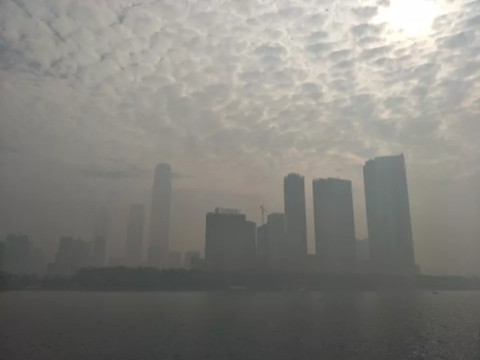
\includegraphics[width=6.67in]{images/cw1}

有人说发展的问题会在发展中解决,例如发达国家也经历过类似的阶段,但伴随产业转型与法规调控,污染问题都会自然而然地消亡;又有人说虽然城市会被雾霾笼罩,但从统计数据上看居民平均寿命其实比所谓田园风光的乡村更长;还有人说大气污染相比土壤、水还有固废污染都不算严重,只是可见度更高(也就是能见度低)\ldots{}\ldots{}的确,雾霾这个现象背后有着错综复杂的社会经济影响,从不同的角度去看会发现不一样的东西。多一个角度看问题并不会让你过的更好,但至少更明白些。

下面我将给出一些非技术与法规调控的视角,希望对读者理解雾霾以及其他一些环境污染问题能有帮助。

\subsection{研究增长的极限}

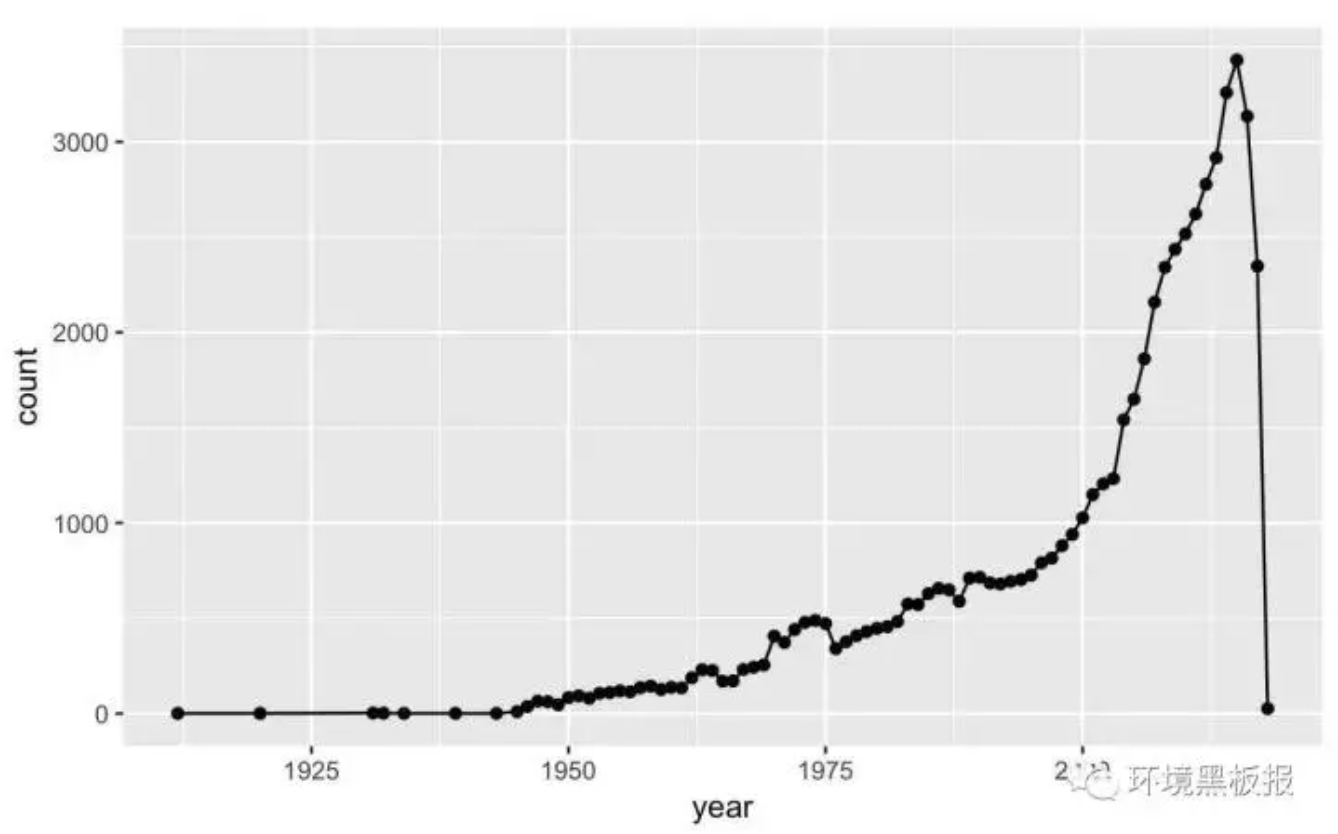
\includegraphics[width=5in]{images/cw2}

上图是生物资讯数据库 Pubmed 上用颗粒物(particulate
matter)作为关键词得到的论文数量,一百年来可以说是持续增长,特别是21世纪以来增长尤为迅猛。但需要注意的是到2015年达到了峰值(3429),16年已经明显下降(3134),今年还有两个月(2348),但不出意外也不会超过16年。至于为什么会有少量18年文献(26),这是学术界硬通货论文的通货膨胀,透支未来可以说是现代社会最伟大也最危险的发明,学术界亦然。也就是说,对于颗粒物的研究兴趣实际已经在降低了。

这个现象可能有点反直觉,因为近几年大气环境污染的公众关注度非常高,经费投放也很可观,但学术界却降低了学术交流频次。无独有偶,使用传统研究热点例如汞、铬、二恶英、基因组、纳米颗粒去进行检索,都会发现研究在2014-2015年间出现了峰值。但同时如果去看一些新兴研究例如3D打印,颗粒物中的细颗粒物(fine
particulate
matter),则增长还是非常迅速的(下图是以细颗粒物为关键词的文献发表状况)。

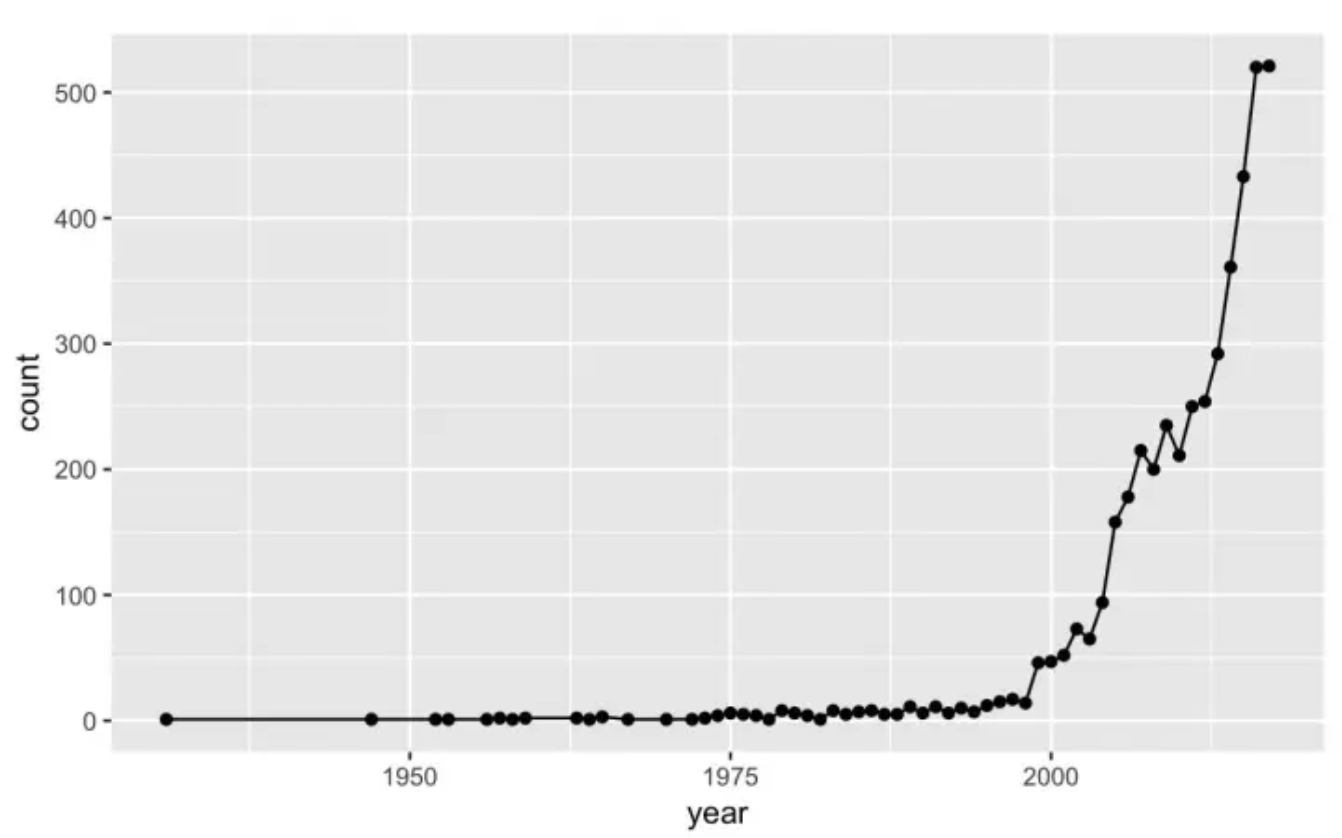
\includegraphics[width=6.67in]{images/cw3}

如果把学术界所有人的研究精力看成是总量稳定的,那么论文数可以看成精力的指标,对于包括大气颗粒物在内的很多环境研究课题而言,学术界正在把蛋糕切给更新的技术与概念。同样是进行雾霾研究,如果你从事微米尺度研究,而学术界却更加认可纳米尺度的研究,那么你的文章就很难发表,然后就是经费紧张,如此循环;进而使得新概念也不断变成老概念。

就颗粒物研究而言,目前学术圈总体关注度已经在下降,但分支中却有上升的。那么可想而知,学科内存在激烈竞争,并不是所有的颗粒物研究方向都是热点。而且还可以预期的是少数研究方向的异军突起会吸收更多学科内的研究资源,很多优秀的研究人员可能一开始选错了研究方向,最终的结局就是转行。研究的增长极限是客观存在的,所以如果你在这个年代打算去找专家咨询,最好去问上升期的新人,因为很多概念从出现到流行不到三五年,有经验的专家反而可能因为有学科内竞争关系而给出带有其自己都意识不到的感情色彩的论断。

\subsection{有原罪的雾霾}

如果某天PM2.5爆表,然后你又恰好感觉到嗓子不舒服,那么很自然你会认为这是雾霾的锅。这符合情理,但不一定符合事实,雾霾跟健康是有联系的,但跟健康有联系的可不仅仅是雾霾。即使仅仅考虑大气污染,颗粒物也只是能够产生爆表AQI的一个因素,其余的例如工业主导的硫酸型烟雾或汽车尾气主导的光化学烟雾都会影响健康,都能让嗓子不舒服,此时你会把原因归到哪里?

进一步讲,环境因素也只是影响健康的一个方面,遗传也起作用。假如你在雾霾天听到一个有气管炎家族病史的患者在咳嗽,你会认为是环境影响还是遗传作用?而根据最近Science的一份研究,即便你排除掉环境因素与遗传因素,仅仅是新陈代谢过程中DNA的复制次数就可解释癌症的发病率的66\%,而这个过程根本就无法用先天后天因素来解释,就是个生长问题。

在中国,雾霾是有原罪的,它实际承载了社会转型期人们的一部分焦虑。如果其对健康的总影响是十,那么其中真实作用可能也就二三,替遗传和其他污染物背了三四的锅,还有三四则可以说是心因性的。今年柳叶刀上一篇文献就提到,中国PM1跟PM2.5大概贡献了医院急诊的4.47\%与5.05\%。这种研究有两个问题,第一,即使排除了意外导致的急诊(例如车祸),就诊行为本身就会受天气影响;此外就是
type M
型错误(效应数量级错误),也就是说这个效应是真实的,但是影响不一定大。

这其实是目前环境研究的一个通病,找一组病人和一组正常人(有的连这个也省了)采集样本,然后一把测定几百上千种污染物(这个现在技术上是没问题的),然后算相关系数,这种情况随机你都可以发现几个的,而这样做出的发现有个通病,那就是效应通常不大,很难重现。一个小而真实的效应或许有学术价值,但舆论一放大就会产生公众心理焦虑,而心理状态又会影响生理状态,这类影响可能并不比真实影响小。

雾霾是有原罪的,但被过度聚焦了,由此产生的焦虑与恐慌本身也会产生健康影响。如果公众可以更好理解科学研究现状与其中的问题,这并不能客观降低空气污染的健康影响,但在实际意义上却可能减轻雾霾的心因性副作用。

\subsection{万金油的幻象}

不知道从什么时候开始,万金油的心态重新出现了。以前如果我告诉你有一种方法可以让你永远远离雾霾危险,你肯定说我瞎扯。好,现在我换一种说法,在人工智能+区块链+可穿戴设备+大数据的实时监控下,我可以给你一副智能眼镜,上面会实时反应你现在的风险指数,如果指数超过80\%,那么你就应该进入室内。逻辑上来说,如果你按照超过指标就躲到室内,那么这个风险永远不会变成100\%,也就是说,这跟我刚才说的永远远离雾霾危险实质等同,但是这样的产品你多半不会觉得是瞎扯,甚至会愿意付高价购买,这又是为什么?

万金油思维从来都没远离过我们,只是从熟悉的名词变成了看似专业的术语。人们有一种看起来很理性但又很荒谬的行为:乐观而盲目地相信着未知的科技。雾霾来了,那就买个最好的空气净化器;外面看不见了,那就来个3M口罩;嗓子不舒服了,那就去搞点清肺的保健品。其实很多人都知道这些科技可能还不成熟,但只要花钱了就有种事情完结可以甩锅的想法。真实的情况往往是越是大家关注的事物,就越有人去贩卖这种包装过的万金油,你买到的更多只是一个确定性的心态。


\includegraphics[width=6.67in]{images/cw4}

在这个分工细致的现代社会里,绝大多数的服务业出售的都是经过专业化包装的确定性,用来抵消分工后一颗颗螺丝钉无法感知全局的焦虑。雾霾就是个全局问题,涉及很多不同专业的知识,当个体被复杂性搞晕时,最简单的方法就是掏出一把钞票买个心安理得。即使问题不能在当前根本解决,但生活总要继续,或许这就是万金油思维在进化上的意义。在雾霾这种大IP下,科学家、政府、骗子、掮客、投机商你方唱罢我登场,过分认真你就输了。

\subsection{混沌的冬日}\label{-1}

回溯千年,宋代诗人陆游在《秋霁》中提到:``驱除云雾极知难'',除了难在技术与法规,雾霾也是直指人心的。

看看窗外,凛冬将至


\includegraphics[width=6.67in]{images/cw5}

作者:yufree 编辑:栟

\section{幻化残生}

幻化残生,也就是环境、化学、材料跟生物这四大学科的近似谐音,都属于实验比例比较高的专业。这些专业的研究生生存现状都------并不乐观。

\subsection{现状}

首先,这四个学科属于建立在脑力劳动之上的体力劳动。例如前处理、过柱、表征、养细胞、涂板子、野外采样等等,流程性非常强,到时间点上不论节假日还是凌晨饭点都得待命;但有时又会发现这些工作找个本科生带上两天也能做出来。一个尴尬的事实是,实验学科一个重要研究方向就是取代人工操作实现流程自动化与便携化,当实验简单到轻轻一按时,研究生训练得到的技能瞬间贬值,更尴尬的是实现这个过程需要的背景知识是物理、机械跟电子工程而不是幻化残生,掌握某项实验技能短期可以使你取得不错的成果,但长期看几乎一定会过时。

其次,特别拼先进仪器/技术,进而导致平台建设重于人才培养。今年这个技术能发顶刊,明年就可能被取代了;有些特殊资源例如光源没有背景想约个机时难得要命,但如果不进行一些高开支实验可能编辑就直接拒稿;而先进仪器装备的价格往往奇高,所以从经济角度,这四个学科都属于很烧钱的。那么这里的尴尬就是,你的才能可能受限于仪器平台;而从研究机构角度看,投资仪器显然比投资人才培养在初期更有效果,而人才培养初期其实也就是仪器操作。这个没啥办法,现在很多科学问题的回答其实早就脱离了理论导向阶段,而是我有一个问题想回答,但目前技术回答不了,也就是假设早就有了,就等着新技术检验。你去看这些年诺奖,很多是技术获奖而不是理论获奖。也就是说,实验学科比起人才更需要仪器平台资源。

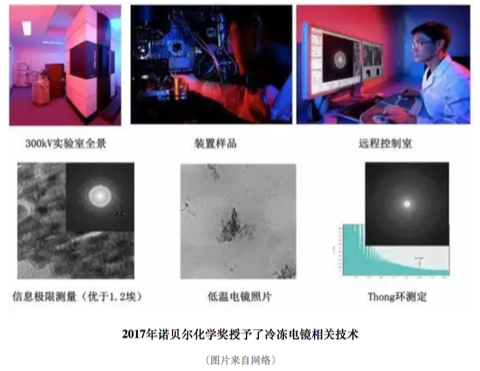
\includegraphics{images/hhcs1.png}

再次,这几个学科产业转化基本停留在前言里,毕业后除了年龄比同专业本科生大了不少,在满足业界要求上本质区别并不大,这进一步导致本应分流到业界服务社会的博士硕士继续留在学术界造纸,而想从学术界熬出头你看前人经验借鉴意义不大。很多人没考虑时代造就的红利窗口期而大谈特谈自己的奋斗,但要知道此一时彼一时,目前学术界的门槛比10年前高了很多,同样的奋斗强度10年前进高校很容易,现在可能去做博士后都没人要了。如果本科转行也就算了,但到了博士转行就真的是在奉献青春了,当然这可能是无法避免的。

\subsection{前景}

我们其实可以把做学术类比创业公司,博士学位前都是导师投天使轮,博士后相当于找风投,找到教职算是有投行介入吹喇叭,常任轨留下来才算上市。论文就像每年的财报,表现不好还可能停牌退市,当然不上市被收购做小老板也行,但那时候学术方向就会完全被大老板把持了。这个过程就是现状,目之所及很多人迷迷糊糊就上道了,而其中沉淀下来的所谓``人生赢家''却没有一个是迷糊的。这里我建议读下
Philip Guo 在斯坦福刚拿到博士学位后写的《The
Ph.D.~Grind》,虽然他是搞计算机科学的,但对幻化残生的研究生了解整体学术圈现状还是很有帮助的,很多观点也会有共鸣。

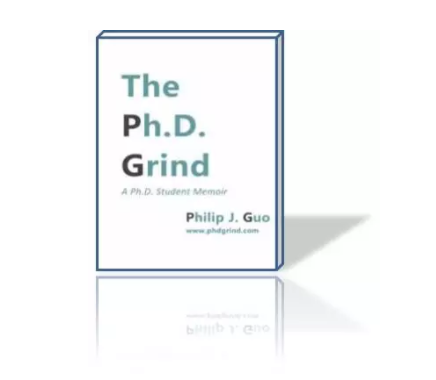
\includegraphics[width=6.67in]{images/hhcs2}

此外,我也可以给出一个基于估计的现状,如果成为院士(中国科学院/中国工程院)算达到学术巅峰的话,那么院士的选拔可以看作到达顶峰的路径。选拔方法是什么呢?两年一次,一次总共大概150人,工程科学对半分,平均一年75人。我们假定若干年后每年还是75人,且平均看每一年参与竞争的都是同年级的博士同学。而目前每年全国土鳖博士毕业生6万多人,算上海归,同一年龄组大概7万人应该比较合理。那么你看到了,你需要在同年级博士毕业生里成为千分之一的精英才算有希望。

这个似乎有点丧气,可能院士这个比较难搞,那么准院士的杰青呢?全国每年选拔200人为杰青,那么成功概率乐观估计是千分之三,杰青其实也很难了,我们再放宽到优青。全国每年选拔400人为优青,那么乐观估计成功几率大概是千分之五。我们大胆认为博士中有一半人毕业后不再从事科研工作,那么几率翻倍成为优青也要是百里挑一。即便是成为教授/研究员,我估计概率也是小于5\%的,这个基数不是所有人,而是跟你同级的博士。

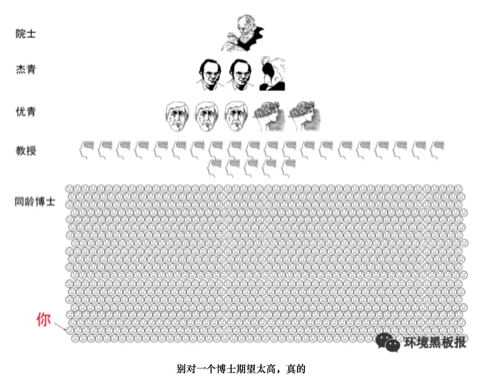
\includegraphics[width=6.67in]{images/hhcs3}

所以其实我挺理解很多劝博士毕业转行或毕业不做学术的看法的,那怕你手握博士学位,在国内想走到教授也是个p\textless{}0.05的事,大概20个人里有一个。考虑到一般博士同学同院系大概也就是20个人,如果学术水平不在前面,基本可以重新考虑下人生规划了,因为此时你选择科研就真的需要兴趣激发了,不然身边的落差会折磨你几十年。而且上面的估计有个严重的问题,那就是大量使用了均匀分布,但真实的情况却是极不均匀分布,你的师承关系跟毕业院校都会把这个分布搞得更加极端,而且后发者优势在科研里面非常常见。同时,目前教职数目趋稳,如果你没赶上窗口期大爆发,基本就是这个竞争强度了,只会更强不会更弱。具体到幻化残生这四个学科中的环境,虽然国家很重视,但在杰青或优青的名单中每年能分到多少个这都是一个巴掌数的过来的,各位可自行倒推下看看竞争强度。如果眼光放远些,其实别的学科的竞争压力也好不到哪去,但对于知识迭代比较快的幻化残生,很多压力与鸿沟可能你没毕业就已经出现了,更糟的是你毕了业才发现。

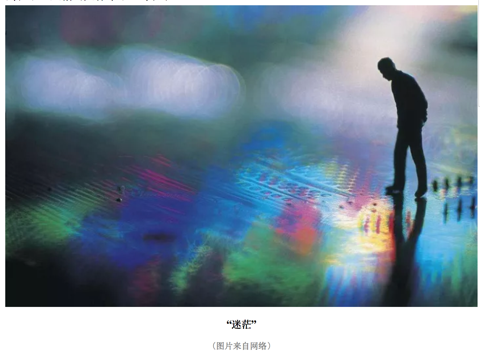
\includegraphics[width=6.67in]{images/hhcs4}

\subsection{求索}

这些现状经常搞得研究生自身怀疑人生,看着转行金融、咨询、IT的同学心有不甘;即便可以用学术理想充实的生活把自己隔离在实验室内,但走出实验室的柴米油盐变量太多,控制不来。同时,你又会很惊奇地发现,这些年报道的学术界年轻有为的青千、优青与各路人生赢家基本都是这四个学科的;而且从经费分配跟论文影响力上看,这四个学科也是超级大户;再从经济学角度去看,你会发现围绕这四个学科的仪器、耗材甚至样品测定跟论文润色服务都已经形成了成熟产业链,行业利润十分惊人。注意,这些产业是对科研进行支撑的而不是业界,如果只是这些行业高速发展而产业界没有起色,那事实上是在用纳税人的经费吹肥皂泡,不会长久。

这并不奇怪,实验学科的知识与技术更迭速度是非常快的,从走进实验室那一刻,你就会发现师兄师姐用的技术学校里根本就没教过或仅仅做了个展望,系统的学习基本上都被传帮带模式替换。如果你自己不去问为什么,大概率你师兄走的弯路你还得走一遍,你师姐画不出的图你也画不出来。更尴尬的是,有时候你会发现,如果你的想法是属于排列组合出来的,那么其实仪器公司完全可以替你做,他们不做并不是不会,而是等着收服务费,你发你的纸,我赚我的钱,各取所需。在这个场景下如果还没意识到自己的民工本质,那大概率是要做一辈子民工的。

曾经有人提过学术界存在生态位,大家各做各的相安无事,但这个想法现在看比较天真,因为现在竞争者基本都不是来自学科内,而是其他学科的入侵,如果这个问题你自己学科的人搞不定,别的学科就会过来。例如做材料的发现一种新材料,如果你觉得意义不大不掺合短期没啥问题,但做材料的表征完了得找应用出口啊,环境、生物、化学都有,技术有自己的生命力,总有人会转过去。你是无法约束某种研究只去关注自己学科内的问题的,事实上这可能是目前科学进步的一个范式:个别学科突破,带动其他学科发展。

基础学科对新技术的接受度要快于应用学科,一个常见的模式就是某个数学模型首先应用在物理领域,然后化学,然后生物,然后是边缘综合学科例如环境、医学,然后就是社会科学。当然也存在某些从应用角度出发的模型后来被应用到其他领域,金融与生命科学中经常出现这样的案例。但你应该发现一个问题,要想解决现在的问题,通常老路是不通的,要么回归基础学科,要么从别的学科借鉴,不论哪一种都需要你持续学习新知识,特别是外学科知识。有一个最简单的办法就是你去看看那些最聪明的人在用什么,然后想想能不能用到自己的学科框架里。

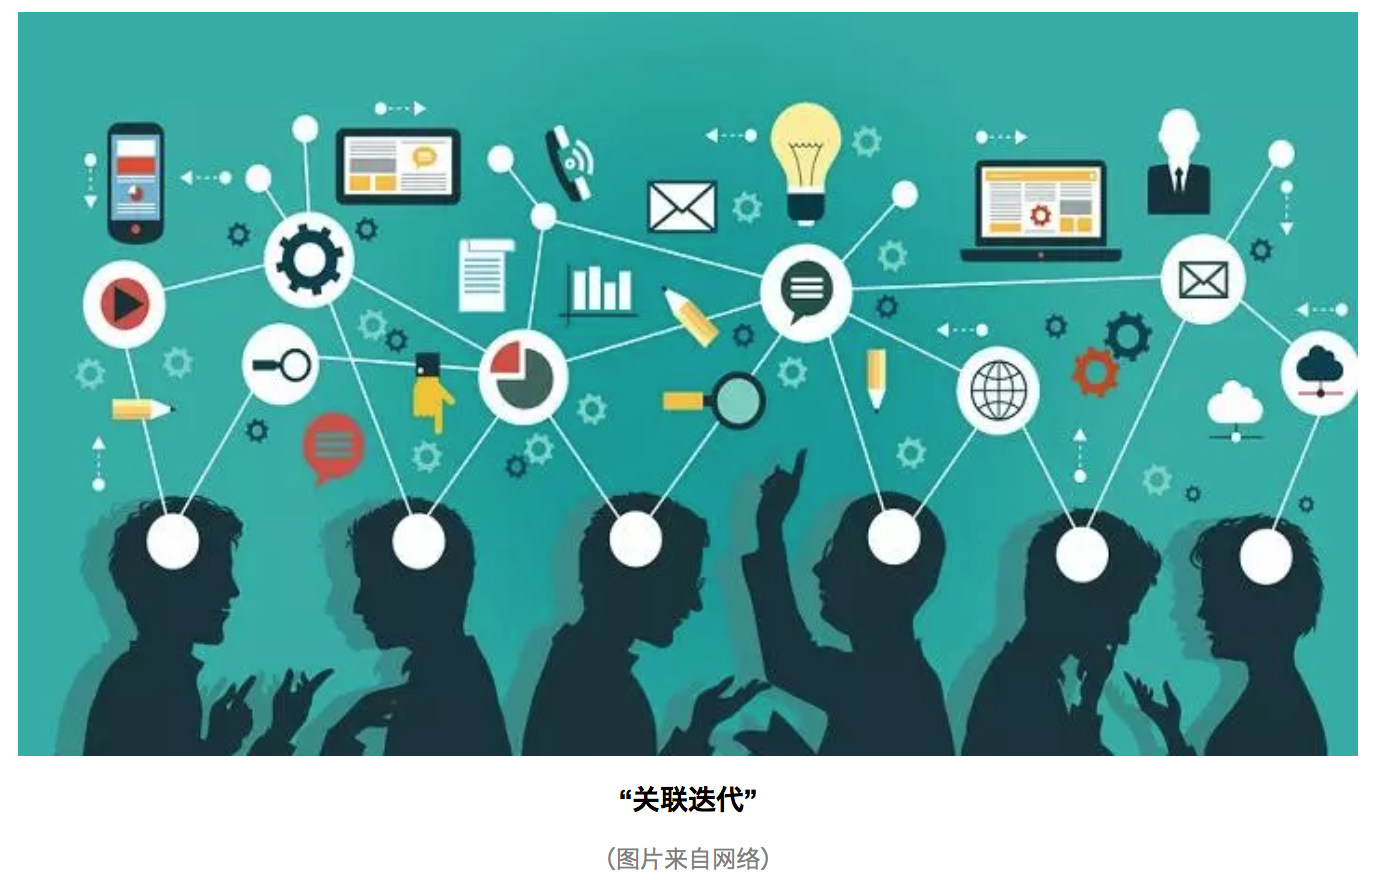
\includegraphics[width=6.67in]{images/hhcs5}

实验学科的发展有时候是很残酷的,初期势必牺牲掉一批掌握过时技术的研究生,这个国内外都很常见。通常国外业界会吸收一部分且通过较成熟的职业教育与培训体系来解决问题,国内则是依靠学术界大面积收留;这个问题的后果就是现在很多教授对于学生无力指导,看到概念就回来让研究生试,研究生自然苦不堪言,毕业后就业方向非常窄。但同样是实验学科,高能物理、生物统计的毕业生转行就相对容易些,因为可以去做码农,至少生活水平对得上学位。而很多实验学科的研究生对此并不感兴趣,甚至完全不懂,思想上停留在努力实验发论文拿教职的简单规划上,不喜欢接触社会就只接触仪器。这其实是最大的偷懒,科研是需要脑力持续投入的,如果是实验学科还要加上体力。不但要持续学习,还必须要主动学习,关心前沿,而这又与繁重的实验任务竞争着的研究生们的精力。在前沿知识的探索中没有固定的方法与理论,经验主义横行,也恰是前沿科研的魅力所在,混杂了无穷的乐趣与苦涩。

\subsection{前沿}

学科前沿是一个很模糊的东西,对幻化残生而言,教科书上的实验技术是一定落后于科研的,此时对学术前沿的感知往往要么来自文献,要么来自会议或培训,坦白说,这两个方法都具有很强的主观性,夹杂很多人的小算盘。好比你想在微信里打开淘宝链接,不是不行,就是要通过复制过程恶心你一把,但其实这种经验过程你也没啥办法。

除此之外,还有一个方法是各种文献信息学指标,例如H指数,被引率等等,但这些指标属于后验指标,你得至少等文章发表过去两三年才能开始评价,但这两三年中也会有一大把新趋势出现。另外一个方法就是自己当期刊编辑或审稿人,其实这个是很多教授的独门秘笈,因为你会比其他人早好几个月知道新研究的动向,但研究生拿到的审稿机会本来就少,高水平期刊更是不会找研究生审稿。所以其实对于很多研究生而言,想了解前沿跟他人的研究动向几乎不可能,而根据我的观察,如果同行坐到一起聊天你对新动向一无所知,那么对方也就不会在你身上浪费时间了。有些出版方跟研究机构也会发布一些热点文章,但多数基于编辑经验,并不一定准确。一个相对靠谱的方法是借鉴搜索引擎排序的思路,通过文本分析的角度从统计模型上探索趋势,这里并不是说那种通过词云这类描述性统计量,而是基于主题模型、时序分析等手段的探索分析,但手段其实是次要的,是服务你的问题的,如果问题没搞清楚,用什么都是错的。

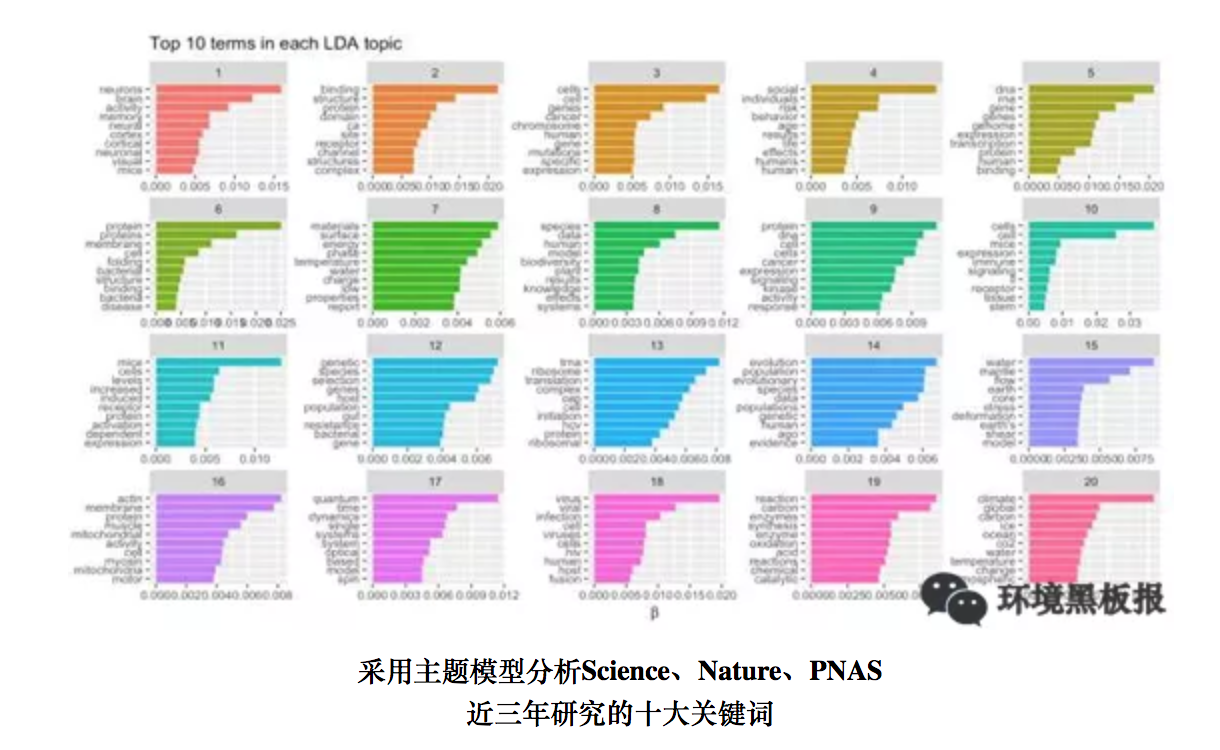
\includegraphics[width=6.67in]{images/hhcs6}

其实,对于幻化残生的研究生而言,主动了解科研趋势只是一方面,了解你自己才是更重要的。当你觉得不好时,不要总是怪罪时代跟环境,也想想自己身上的问题;当你一帆风顺时,不要总觉得这是自己勤奋与努力的结晶而忘记了科研浪潮的背后推手。随波逐流不会过的太差,但放弃思考是绝难在学术界生存下来的,不要真的幻化残生了。

师兄只能帮你到这了,剩下的,我也没想明白。

本文首发于我的科学网博客(yufree),改编首发于环境黑板报。

作者:yufree 编辑:栟

\chapter{城市生态}

\section{城市之殇}

\subsection{序言}

2012年7月21日,一场61年一遇的大暴雨让北京成为``汪洋水城'',想不到有生之年居然可以在帝都这个缺水的城市同时实现了``山盟海誓''。无独有偶,不仅北京遭遇了这样的窘境与困惑,其他城市诸如南京、武汉、广州、杭州等也先后开启了``看海模式'',这种``城市之殇''已经成为近年来城市发展挥之不去的阴影。

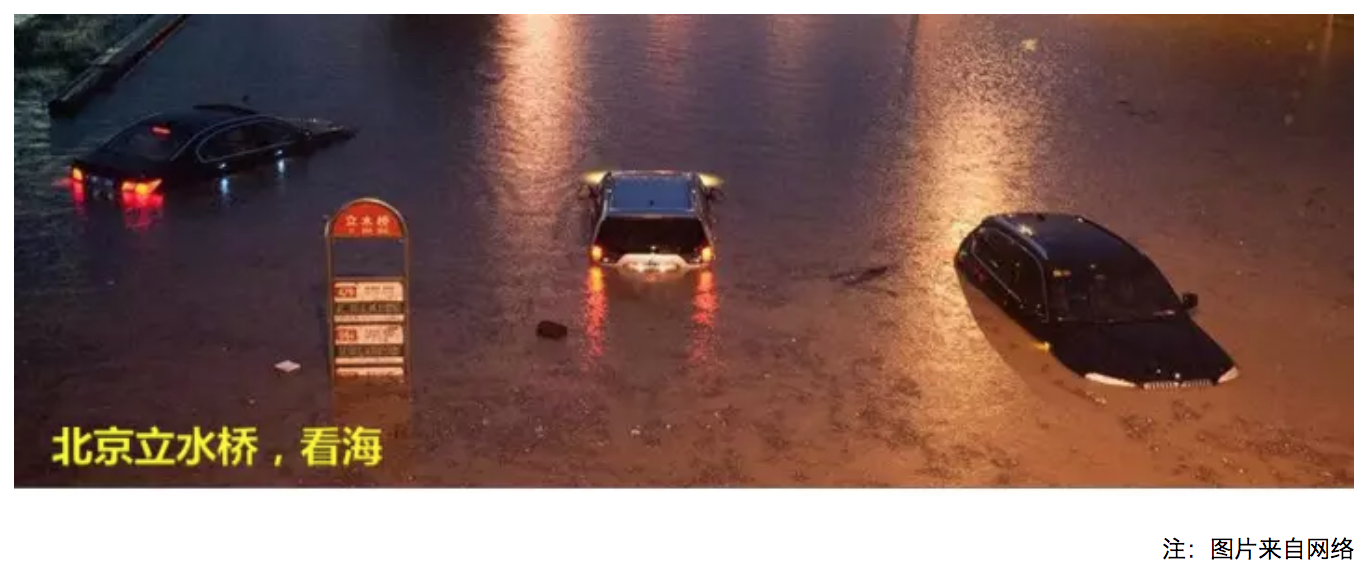
\includegraphics[width=6.67in]{images/ch1}

那么,为什么我们城市的排水能力一遇到暴雨甚至中小雨就原形毕露?这就有必要来聊一聊本期的话题:``海绵体''。海绵体,顾名思义,是一种对蓄水的形容,自然界原本是一个巨大的海绵体,而如今城市的爆发式发展建设已严重破坏了自然的海绵体,损害了自然的水循环系统。传统的城市建设模式根本不具备应对超标雨水的能力,那么必然会导致``逢雨必涝'',同时还会带来水环境污染、水资源紧缺、水安全缺乏保障等问题。

2013年12月12日,习近平总书记在《中央城镇化工作会议》的讲话中强调:``提升城市排水系统时要优先考虑把有限的雨水留下来,优先考虑更多利用自然力量排水,建设自然存积、自然渗透、自然净化的海绵城市''。海绵城市顺应时代号召应``运''而生。

\subsection{海绵城市是什么}

海绵城市的理念其实在我国古代早已践行,比如故宫的排水系统、云南的``哈尼梯田''模式、赣州的``福寿沟''蓄排系统等,都算作是早前的雏形。若要刨根求底地问海绵城市是什么,海绵城市更多的是一种新型的城市发展模式。

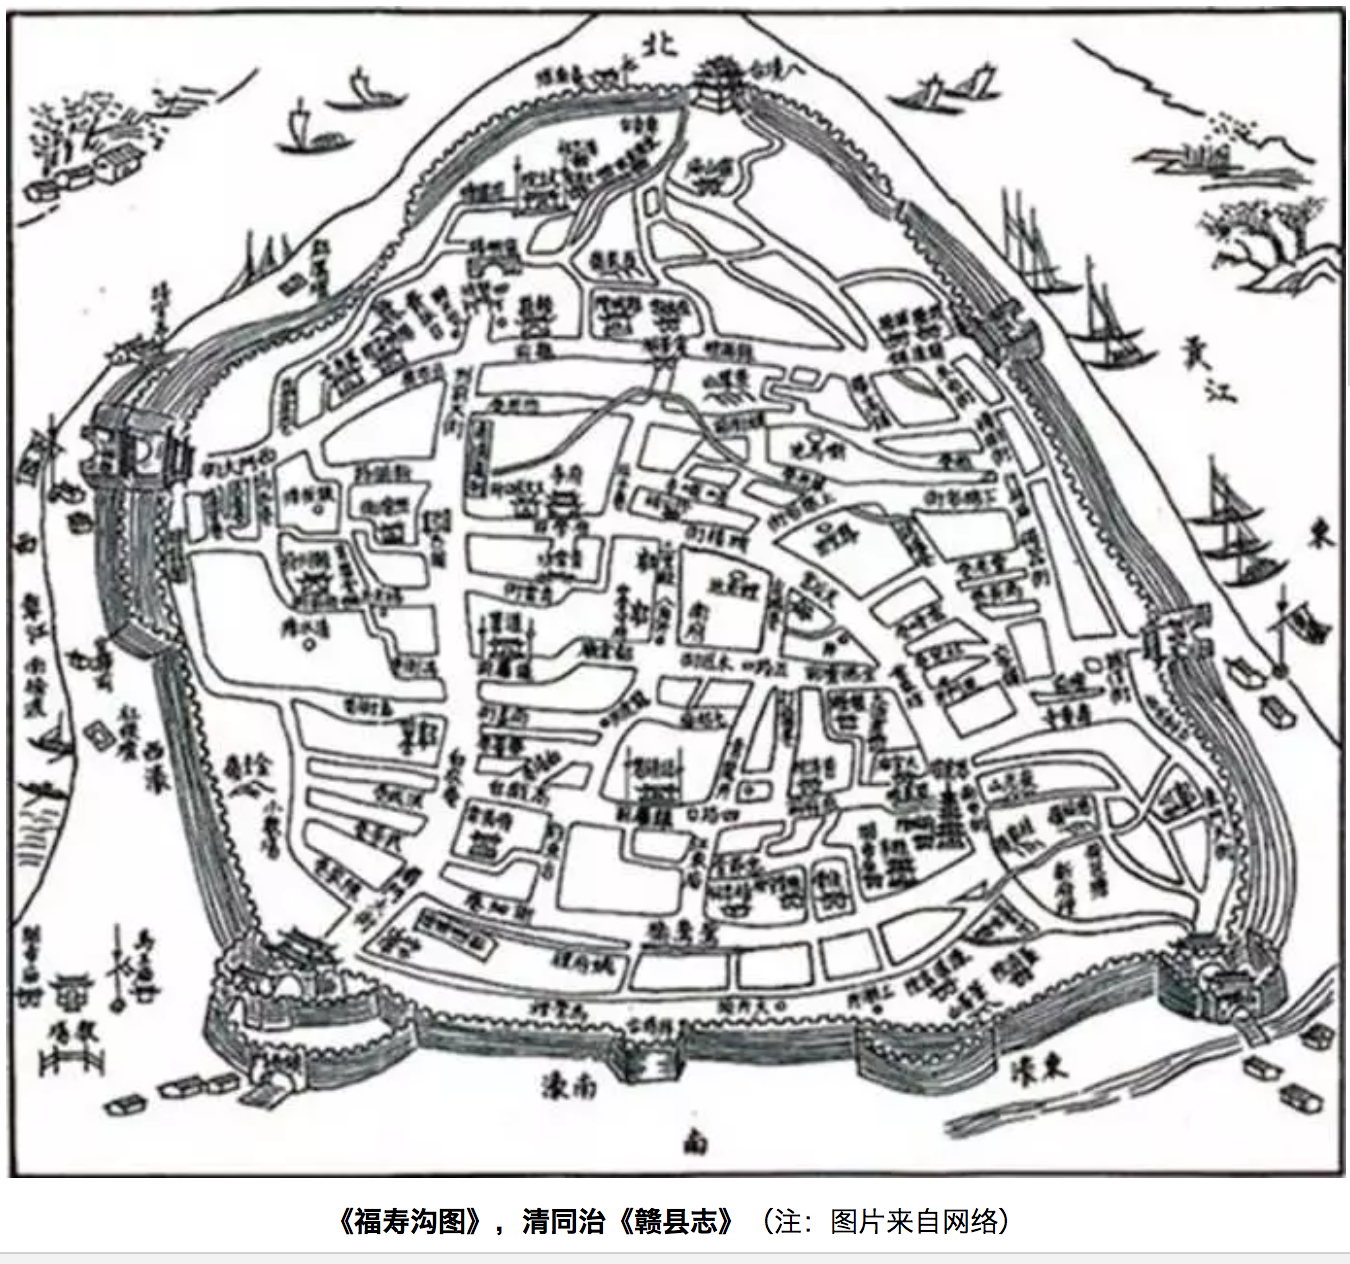
\includegraphics[width=6.67in]{images/ch2}

海绵城市的初衷是让城市能够像海绵一样,在适应环境变化和应对自然灾害等方面具有良好的``弹性''。简单来说,下雨的时候,城市可以像海绵一样吸水、蓄水、渗水,防止洪涝的出现;在雨水过后,干旱的时候,又可以将蓄存的水``释放''并加以利用。但同时,我们又希望这个``海绵''能发挥更大的作用,比如说还可以净化水体,让雨水在城市存积、渗透的同时得到净化,以利于进一步的雨水资源利用和生态环境保护。这就为海绵城市的设计、建设提出了更高的要求,不单是依靠恢复或构建自然途径来蓄水、存水,还应当结合人工措施来辅以完成水资源的净化、利用和排放。

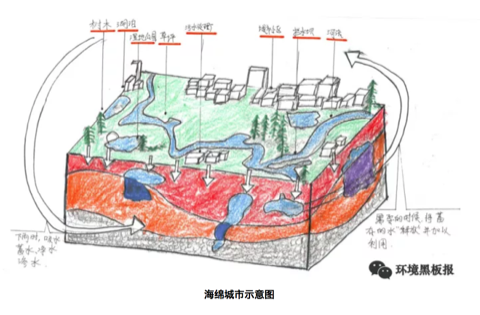
\includegraphics[width=6.67in]{images/ch3}

因此海绵城市的具体建设既不能``窄'',也不能``宽''。太窄就会回到植树造林搞绿化的老路子上去;太宽就会变成``海绵城市一个框,啥都可以往里装''。其实海绵城市建设还是要以目标与问题为导向,运用``源头、中途、末端''的措施,使绿色设施与灰色措施相结合,才能实现真正的目标。

简明地讲,源头主要以低影响开发设施(LID)为主,包括植草沟、雨水花园、生物滞留设施等,中途主要包括:雨水廊道、管网、沟渠等,末端主要包括:湿地、调蓄塘、调蓄池、水系等。

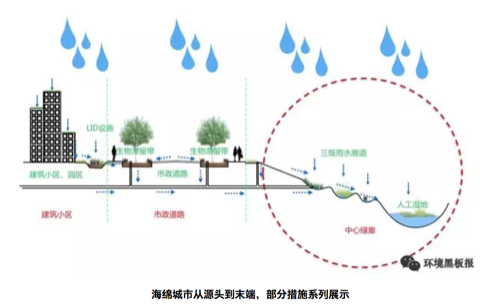
\includegraphics[width=6.67in]{images/ch4}

\subsection{海绵城市试点}

海绵城市的建设借助国家重视生态环境的东风,目前共执行了2个批次、30个城市的试点,试点期3年。期内国家将给予直辖市每年6亿专项补助,省会城市每年5亿,其他城市每年4亿元。

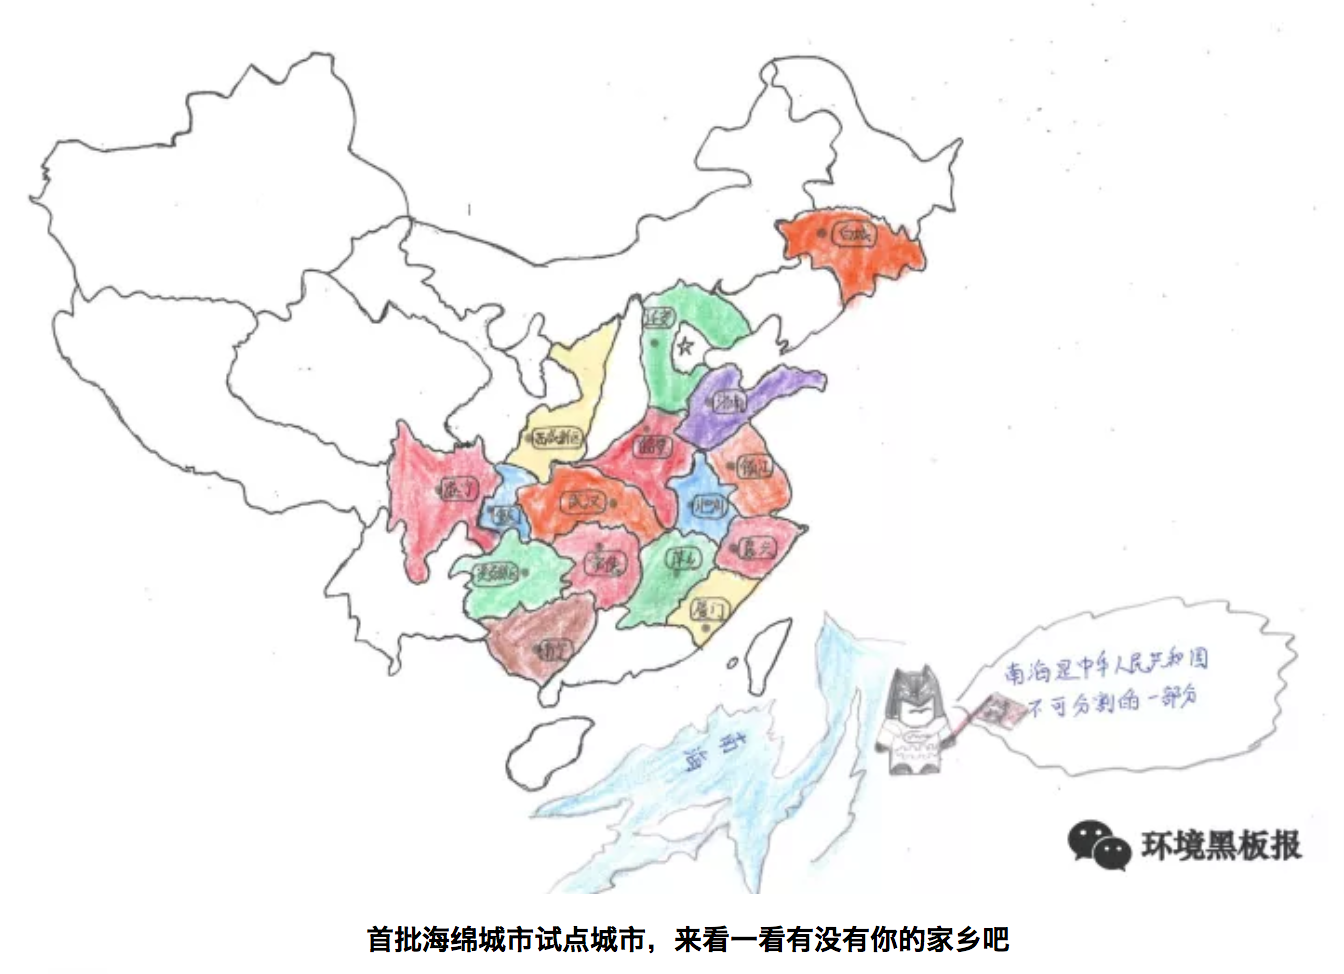
\includegraphics[width=6.67in]{images/ch5}

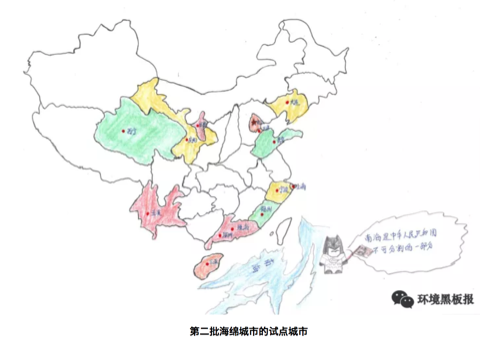
\includegraphics[width=6.67in]{images/ch6}

目前来看,海绵城市建设还没有一个全国性的``统一标准'',主要是因为我国地域差异大,东西南北中,面临的问题与挑战各不相同。比如北方地区多为缺水的寒带地区,南方地区则更容易发生内涝,西部地区多属于湿陷性黄土地区,也极度缺水。因此不同区域的海绵城市建设也应因地制宜。

\subsection{浅谈海绵感悟}

笔者从2015年开始从事海绵城市建设方面的工作,先后参与了多地的海绵城市试点建设的咨询、设计等工作,主要涉及海绵城市建设系统方案编制等方面。这里跟大家分享一下三年多来笔者对海绵城市建设的一些想法与感悟,希望能对现在或将来参与到海绵城市建设中的同仁们有所帮助。

\subsubsection{从管理部门的角度}

如果您是一位相关部门的负责人,笔者虽人微言轻,但也愿意提供一些思考供您参考。
海绵城市的建设是一个很复杂、庞大、时间跨度也大的系统工程。而且里面涉及到很多学科和部门,简单数数就需要规划、市政、园林、水利、道路等专业;住建、水利、园林、环保等部门来互相配合。因此如何统筹规划,通力协作,避免形成各自为政、``九龙治水''的局面,是一门很深的学问。

同时,很多城市现在都有新、老城区,新城区建设制约少、阻力小,一旦方案设计得当,大可一马平川。但是老城区就不一样了,不仅居民多、遗留矛盾和问题多多,牵一发而动全身,搞不好容易激化矛盾。这个时候,就不能只顾海绵城市建设的目标,还要考虑经济承受能力、轻重缓急、资金利用效率、建设时序、社会影响等方面。
千万、千万不能不分轻重地全面开工建设和盲目翻挖。最好可以以解决城市内涝、雨水利用、黑臭治理为突破口,结合棚户区和城乡危房改造、老旧小区有机更新等工作同步推进。

\subsubsection{从项目公司负责人的角度}

当前海绵城市的建设基本上都以项目打包的形式交由PPP公司全权负责建设。如果您是一位项目公司的负责人,首先恭喜您拿下了海绵城市的项目,但是接着愁人的事情来了。在很多项目管理过程中,一些PPP公司``当家不做主'',没有自主权,项目的管控不是由PPP公司独立操作,而会受到相关部门的干预,导致指挥不合理的局面。因此,如果您能在项目开展前和相关部门做好充分的沟通,对您后续工作的开展会有很大帮助。
同时,虽然目前海绵城市都处在建设之中,但是即使这样,试点期也已经过了2-3年,后期的运营维护也该做一些考虑了。如果您公司还没有做这方面的准备,那可千万要小心了,现在环境追责可是很严重的哦。

\subsubsection{从设计师的角度}

如果您是一名规划师或者设计师,请一定要``迈开腿,管好嘴''。一定要多去现场,没有调查就没有发言权,不能板凳一坐就站不起身,嘴皮一碰就出方案。曾经有一位设计院的设计师理直气壮地反驳说没必要去现场看这么细,走了个过场回来,后来设计的时候全部依靠业主来提供信息作为依据。结果可想而知,做出来的设计方案根本经不起推敲,漏洞百出,更别说拿去指导施工建设。

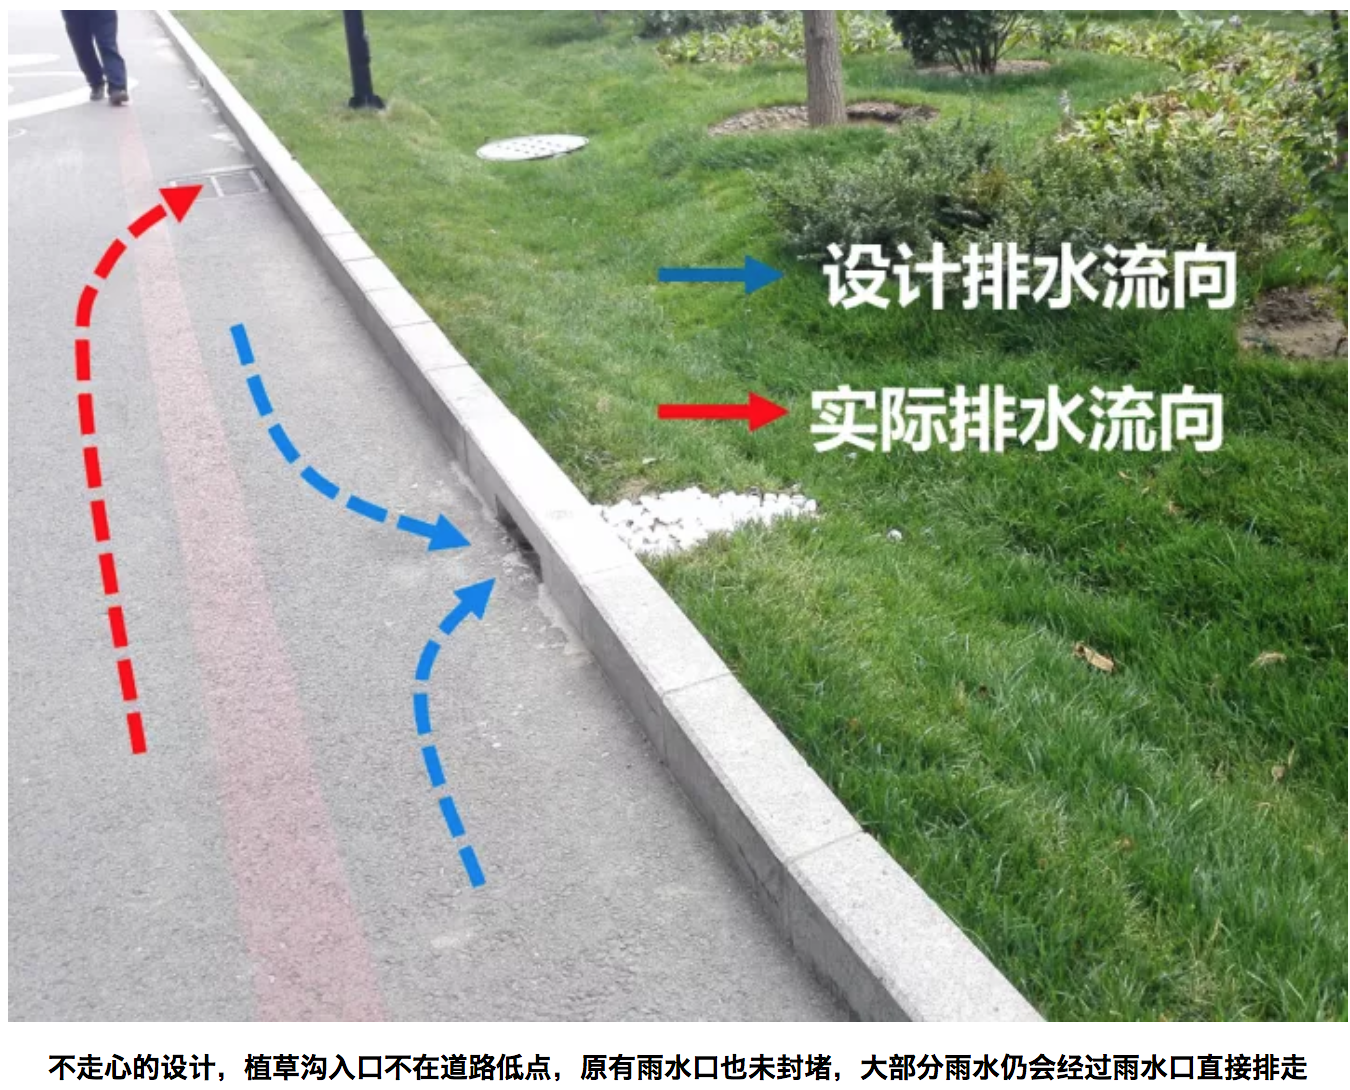
\includegraphics[width=6.67in]{images/ch7}

同时也提醒大家,海绵城市建设不只是``搞种植、搞绿化''。``花花草草''固然重要,但我们也不能天天搞``拈花惹草''的老一套。海绵城市的实质应该是绿色设施(雨水花园,植草沟,下凹式绿地等)与灰色设施(管网,泵站,调蓄池等)相结合,让它们在不同时间与空间上起到相应的功能与作用。

\subsection{结语}

海绵城市的概念一经提出,就在全国迅速地铺展开来。国内新事物的出现,不像国外``自下而上''的推进模式,而是``自上而下''的运动式推动。然而,没有前期多年的研究数据作为支撑,直接开展工程实践难免会面临各种各样的困境。
目前,``海绵城市''的提法基本已家喻户晓,无人不谈``海绵'';然而能真正潜下心来认真对海绵城市进行系统的研究与梳理的人却少之又少。一个新的领域,往往需要十年甚至更长的时间来形成系统性的理论与技术体系,之后才有可能更高效、更全面指导工程实践。希望各位海绵同仁,我们一起潜心努力,为这个领域尽自己的绵薄之力。

作者:王宇 校稿:广播站王站长 编辑:栟 手绘美图:丫头晚安

\section{污师私房菜之OUR 和 SV30 的应用}\label{our--sv30-}

在污水处理领域,活性污泥工艺可谓无人不知无人不晓。活性污泥吃着排泄物,干着体力活,最终为我们产出清水,真乃当下``撸起袖子''的楷模。说到活性污泥真是让人既爱又恨,爱的是它能帮我们处理污水,恨的是它不善于表达,和人类语言识别系统无法链接,当污水处理系统出问题的时候,初入运维界的你却无法第一时间判断活性污泥究竟为什么罢工,只能求爷爷告奶奶的到处请教大神。


\includegraphics[width=6.67in]{images/os1}

今天通过\textbf{活性污泥呼吸图谱}和\textbf{污泥沉降性比}的应用介绍,通过熟练掌握这两个污水处理厂运维秘籍,让你可以和活性污泥随时交流,对污水处理厂的运行维护清晰把脉,及时准确解决出现的问题,让你的格调得到迅速提升,变身污水处理领域的运维大神。

\subsection{呼吸速率的前世今生}

话说20世纪50-70年代,国外有一群水处理界的大神(Eckenfelder,Mckinny,Lawrence-McCarty)闲着没事东看看西瞅瞅,就弄了个活性污泥模型出来,在里面就提到了\textbf{呼吸速率}(Oxygen
Uptake Rate,
OUR)的概念。所谓\textbf{呼吸速率是指单位时间内活性污泥消耗的溶解氧的量}。呼吸速率的概念由来已久,关于测量呼吸速率的专利也是层出不穷。然而呼吸速率一直应用于模型理论层面,在实际指导污水厂的运行方面却是凤毛麟角。(如何测量OUR就不在这里赘述了,请大家自行查阅相关秘籍)

我们知道在活性污泥工艺中有两种主导微生物:异养微生物和自养微生物。\textbf{异养微生物}需要消耗外部碳源维持自身生长(不给肉吃,它就死给你看);而\textbf{自养微生物}就是楷模了,可以通过分解无机物获得能量维持自身生长(真是吃着土,干着活)。这两种微生物都有各自的呼吸速率,异养微生物降解有机物时的呼吸速率称为\textbf{异养菌呼吸速率};自养微生物降解氨氮时的呼吸速率称为\textbf{自养菌呼吸速率}。有时活性污泥闲着无事也会吃些自己身上的东西,把微生物利用细胞内含物质作为基质进行新陈代谢过程中的呼吸作用称为\textbf{内源呼吸速率}。图谱如下图所示:

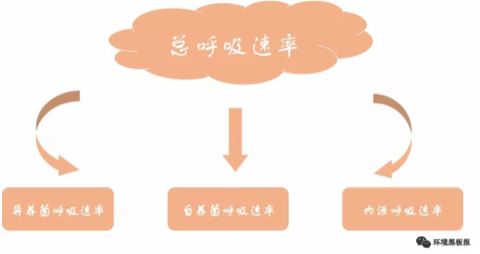
\includegraphics[width=6.67in]{images/os2}

\subsection{OUR应用的理论介绍}\label{our}

上面介绍了呼吸图谱的组成,下面来谈一谈呼吸图谱的作用。为了更清楚的起到对比,我们需要在污水处理厂正常运行时,刻苦用心的你日常闲来无事多测测好氧池OUR,建立一个污水处理厂的OUR数据库,对正常情况下的OUR烂熟于心,只有这样你才能了解你自己一亩三分地的情况。

通常,\textbf{活性污泥OUR值的大小及其变化趋势可对好氧池负荷的变化情况起到预警作用,同时OUR的变化也间接反映出活性污泥自身的健康情况}。我们分两类情况进行分析:

\subsubsection{OUR异常高于正常值的情况}\label{our}

如果OUR若大大高于正常值,表示活性污泥需要消耗大量的溶解氧,表明优秀的活性污泥小伙子们正在撸起袖子加油干,这也往往预示着污泥负荷过高,可能超过污水处理厂的处理能力,这时出水水质可能超标。

\begin{quote}
你可以脑补一下这个场景:一个房间里面有十个饥饿的小伙子,你拿来十个馒头,他们能以迅雷不及掩耳盗铃响叮当之势把这十个馒头干掉,可如果你拿来一千个馒头,就算是吃到怀疑人生也吃不完。
\end{quote}

\subsubsection{OUR异常低于正常值的情况}\label{our}

如果OUR长期低于正常值,表示活性污泥消耗的溶解氧较少。这就需要分两种情况来分析了,一种情况是活性污泥精神抖擞,战斗力强,污染物负荷较小,污染物降解好,出水水质好;另外一种情况就是污泥活性差,污泥本身对污染物的降解性能不良,这可导致出水水质不达标。

\begin{quote}
第一种场景是这样的:一个房间里面有十个饥饿的小伙子,你就给五个馒头,估计最后盘子都会被吃掉;
\end{quote}

\begin{quote}
第二种情况是这样的:同样是这个房间,同样是五个馒头,但是吃馒头的人变成了十个胃口欠佳的病人,结果可想而知。
\end{quote}

\subsection{OUR应用的实战演练}\label{our}

上面对OUR应用的理论介绍还是比较笼统的,下面详细讲解一下如何利用OUR来判断出水水质,针对OUR的应用进行实战演练。

\subsubsection{实战场景1}\label{1}

用心的你费了九牛二虎之力测定了好氧池的OUR,发现OUR值比较低,根据理论分析,你记住了OUR异常低于正常值的第一种分析情况,认为活性污泥小伙子们战斗力强,降解能力个顶个,赶紧跟领导汇报说出水达标没有问题。你刚汇报完,厂里就通知你出水超标了,这脸被打的啪啪响。

这时,你一定会问,OUR值低,说明出水水质好,怎么出水还超标了呢。少年不要急,听我慢慢说来。

在OUR值比较低的情况下出水超标,说明此时的活性污泥并没有正常工作,那该如何解决呢?这种情况下你只需要往装置内部补充\textbf{足够的碳源},最常见的是投加乙酸钠,看看\textbf{投加碳源后的OUR值变化},如果OUR值还是很低,说明你的活性污泥活性差,大多都是老弱病残,再怎么给他们喂食碳源也不能发挥他们的作用;如果OUR值在投加碳源后明显升高,说明你的活性污泥是健康的,他们只不过是饿了,需要饱食一顿接着好好干活。

\textbf{因此,在好氧池OUR值比较低的情况下,判断出水是否达标的时候,需要结合好氧池当下的OUR和投加完碳源后的OUR进行判断,才能准确对污水处理厂的运行状态进行评价。}

\subsubsection{实战场景2}\label{2}

勤快的你这天又测定了好氧池OUR,发现OUR值很高,结合OUR异常高于正常值的情况分析,你下结论说出水水质达标。

少年你又要被打脸了。

\textbf{好氧池当下OUR值高,说明好氧池中污染物负荷高,表明好氧池需要消耗大量的溶解氧,为了保证出水达标,你需要做一系列应对措施,比如增加曝气,减少排泥量等等,只有这样才能保证你的出水达标。}

\subsubsection{实战场景3}\label{3}

就是这么巧,你们公司属于水处理界佼佼者,你一亩三分地里面管辖着若干个污水处理厂,你也坚持着建立了各个污水处理厂OUR的数据库,你也是一个闲着无聊喜欢翻数据的人。有一天,你发现针对不同污水处理厂,即使在进水和出水水质相差不大的情况下,好氧池的OUR差别仍然很大,这时你又迷茫了。

不要迷茫少年,因为在测量OUR时并没有考虑\textbf{污泥浓度}的因素,\textbf{污泥浓度高的,表明污泥中活性微生物较多,OUR值较高,污泥浓度低的,表明活性微生物少,OUR自然就低一些}。你可以想象一下,10个人和100个人的体重还是有很大差别的。

那如何采用一个统一的评价指标来评价呢?我们在污水处理厂的运营维护过程中,善于发现问题的同时,还要善于解决问题。这时,我们引入一个叫\textbf{比呼吸速率}(OUR/MLSS)的评价指标,你就会发现在入水水质和出水水质相差不大时,各个水厂的比呼吸速率相差也不是很大,是不是完美的解决了你的困惑呢?

\subsection{SV30的应用实战}\label{sv30}

上面给大家讲了比较高大上的OUR,接下来再给大家讲讲污泥沉降比的实战应用。SV30,在污水处理界的地位,犹如《天龙八部》中的扫地僧。可谓是量筒在手,天下我有。

做过污水处理的人应该都知道,\textbf{污泥30min沉降性能},可以一定程度上说明污泥的性状,所谓画虎画皮难画骨,具体判断污泥处在哪个状态却不是一件容易的事。可能或许也许maybe只有真正达到扫地僧的级别才能通过SV30一眼识别出污泥的性状来。

少年也不必灰心,鄙人在藏经阁翻阅典籍无数,浏览宝典若干,给大家总结了一些关于SV30的要点。大家理论联系实际,在测试SV30的时候,通过实际观察并结合我提供给大家的要点,相信大家早晚能达到扫地僧的级别。

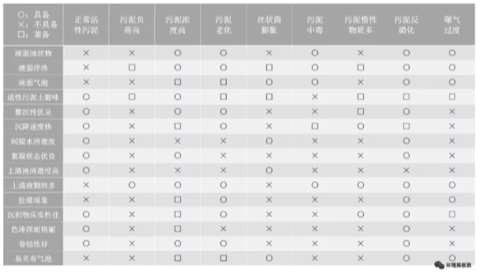
\includegraphics[width=6.67in]{images/os3}

这里告诉大家一个小诀窍,千万别告诉其他人。

在测试SV30的过程中,重点观察\textbf{前5min的沉降效果},活性污泥沉降实验的前5min往往可以完成沉降过程的80\%,此阶段的沉降效果好坏往往可以指导对活性污泥性能的判断。

你可千万别取完样定个时间,先睡他半小时。所谓武功再高也怕菜刀,在测SV30的时候\textbf{量筒的选择}很重要,建议大家选用1L的量筒,量筒过小可能会发生污泥挂壁现象影响效果。再次重申,这些小诀窍千万别告诉其他人哟。

\subsection{结语}\label{-1}

以上算是给大家介绍了关于污水处理的两个秘籍,

一个是修炼较困难的葵花宝典------OUR,

一个是老少皆宜的太极拳------SV30。

所谓难易结合才能事半功倍。当然,掌握了以上两个技能也不能洋洋自得,天下之大,无奇不有,只有不断充实自我,才能屹立在污水处理行业的尖端。

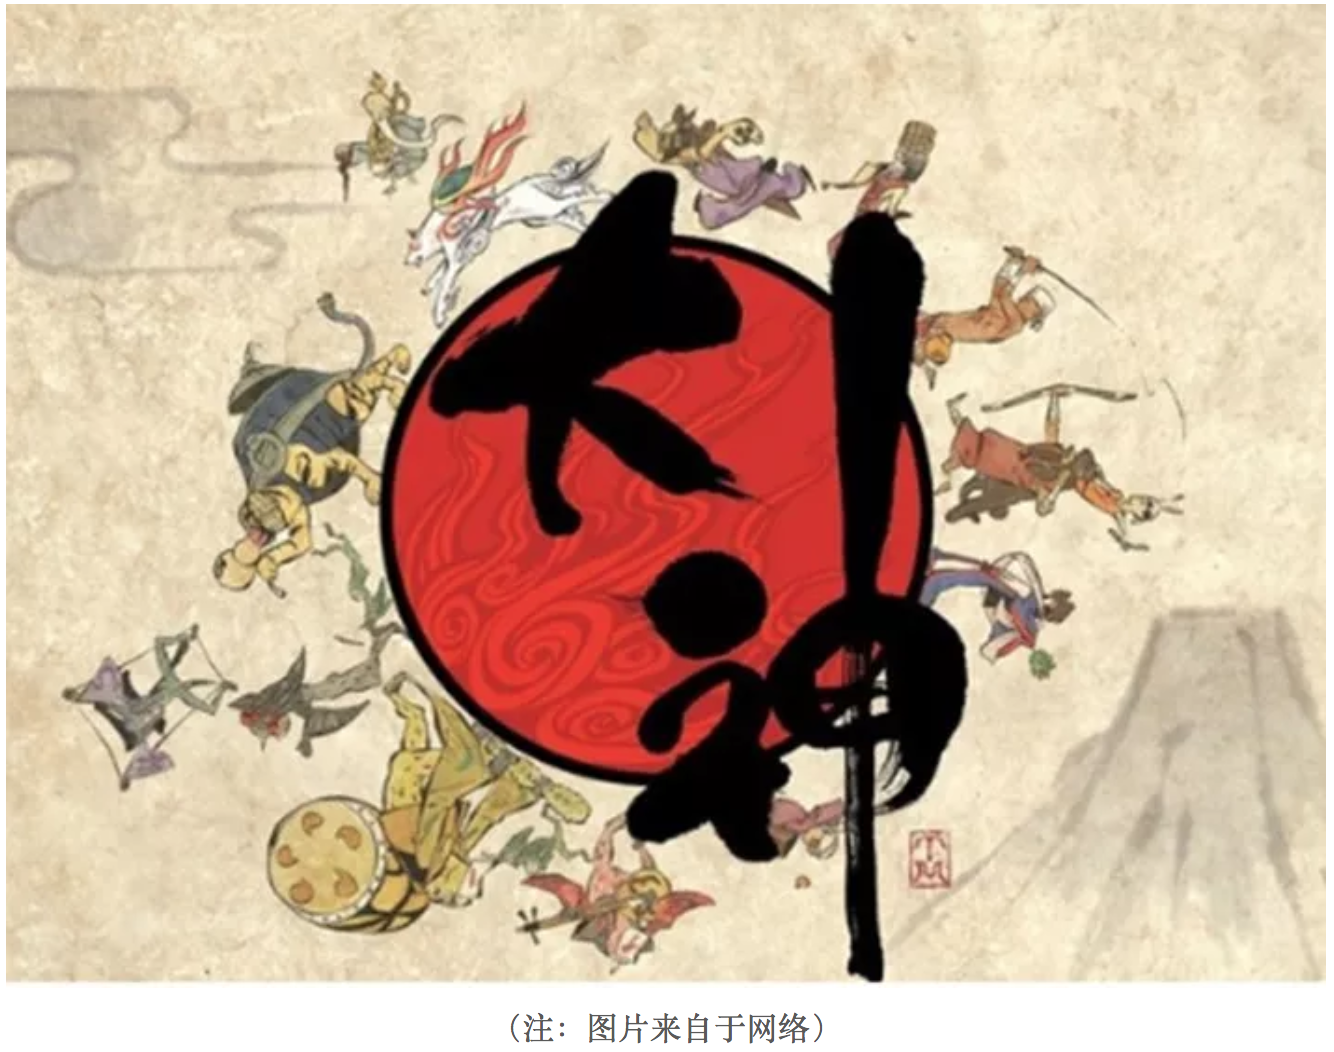
\includegraphics[width=6.67in]{images/os4}

作为一个21世纪的污水厂操作人员,作为一个生活在大数据、物联网、云计算时代的污水厂操作人员,作为一个人工智能正在逐渐取代你饭碗的污水操作人员,仅仅依靠设计规范上面的知识已经难以追上时代的列车了。只有与时俱进,汲取新知识,用知识的力量将命运牢牢把握在自己手里。

成神的道路注定是孤寂乏味的,成神的道路注定是披荆斩棘的,成神的道路注定是一往无前的。少年,抓住当下,紧跟大师步伐,成神指日可待。

作者:阿布呆 校稿:看透, yufree 编辑:智公子 美图:丫头晚安,智公子

\chapter{岸芷汀兰}

\section{听花杂记之晚清四名臣}

作者按:在中国历史上有两个思想动荡的年代,一个是随着分封制瓦解,国家向帝制过渡,整个社会礼坏乐崩的春秋时期;另一个就是晚清。要说来,晚清时代的动荡要远远大于以往任何一个朝代。延绵了几千年的封建制度已经日薄西山,那些祖祖辈辈相传的至理竟然在列强的纷争中无从适用,而新的思想还没有开始萌芽。那无尽的黑暗,给晚清人物的性格烙上了复杂而深刻的两面性,每每读起,都唏嘘不已。

\subsection{胡林翼}

\begin{quote}
挥金如土、杀人如麻、惜才如命
\end{quote}

胡林翼的才华有多大呢?他有一个号,叫润芝,是的,太祖后来取了一个和他一样的字(后因太祖不想被人称作草头司令,去掉了``芝''的草字头------小编按)。这位晚清的中兴之臣是曾国藩最忠实的盟友,也是曾国藩二次出仕前最大的润滑剂。尤其他开创的``夫人外交''极大地缓解了新兴汉人将领和满清贵族之间的矛盾。

胡林翼是湘军将领中最有人情味的人,但他又是镇压太平天国最无情的刽子手。不论流连花间,还是重赏将士,他挥金如土;而面对敌人和对手,他杀人如麻;遇到才华出众的人物时,他又倾心相交,惜才如命。\textbf{``挥金如土、杀人如麻、惜才如命''}胡林翼以此``三如''名动天下,为曾国荃所膜拜,真是好一个屠夫手段、菩萨心肠!

1861年的时候,常年的征战和纵情声色极大地损伤了胡林翼的身体,然而谁也不会想到这位不到五十岁的封疆大吏甚至没能熬过这个秋天。时值九月,岁在三秋,身体有所好转的胡林翼在曾国藩、彭玉麟的送行下由安庆乘船返回武昌,长江上本来一派祥和的气象,忽然一声汽笛声破空而入,抬眼望去,洋人的巨船逆江而上,转瞬间便已经去远。胡林翼悲从心生,竟生生咯出了一口血来。``洋船其快如斯,如若开战,我辈如何能敌?''这一咯,竟就断送了胡林翼的性命。

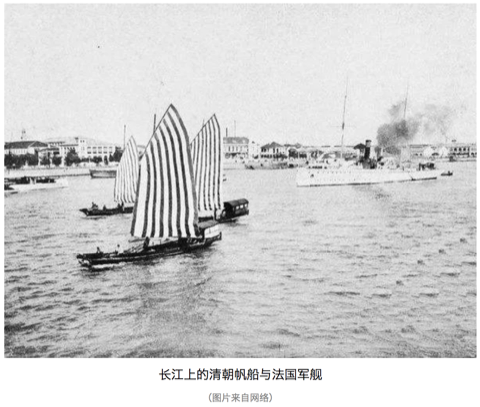
\includegraphics[width=6.67in]{images/his1}

这个故事当然可能是杜撰,而我却宁肯相信这个故事是真的,因为洋务和国家一直是胡林翼的一块心病。这是一种无比深切的怅恨,是一种亲眼所见又知道终其一生甚至往后百年都无法赶超的悲哀。正所谓,哀莫大于心死!这一咯,咯出了多少仁人志士的心声,不管他们有这样或那样的缺点,他们前赴后继,就能顶起中国的脊梁。

\subsection{左宗棠}

\begin{quote}
天下不可一日无湖南 湖南不可一日无左宗棠
\end{quote}

四名臣里,左宗棠的才华是最高的,也是自视最高的,他在给友人的信里,常常署名叫今亮,也就是当今时代的诸葛亮。他一生未中功名,后来以幕僚出道。普通幕僚的命运都是和提携他们的人紧紧捆绑在一起,明朝有一位很出名的文人,叫徐渭,也叫徐文长,他是浙闽总督胡宗宪的幕僚,在擒拿倭寇上曾风光无限,后来胡宗宪下狱,徐文长便开始了潦倒的后半生,成了``南腔北调人''。

然而左宗棠却摆脱了这一命运,他才高不可一世,以举人身份怒斥总兵樊燮的怠慢,却反被恼羞成怒的樊燮弹劾,以至于被定罪下狱,上谕``有不法事,就地正法''。然而,历史并没有放弃这个真正有才华的人。

左宗棠被下狱的事情犹如一石激起千层浪,不仅郭嵩焘、胡林翼、曾国藩等多方保举,探花郎潘祖荫更是写下了足以流传百世的奏折:

``以本省之饷,用本省之兵,不数月肃清四境,其时贼纵横数千里,皆在宗棠规画之中。设使易地而观,有溃裂不可收拾者。\textbf{是国家不可一日无湖南,湖南不可一日无左宗棠也}。''

这段话奠定了左宗棠一生的基调。

19世纪五十年代末,沙俄开始了他们疯狂的领土扩张,他们先后在我国东北部割占了大约100多万平方公里的土地,以至于时到如今,我们还要靠放养大马哈鱼来维持图们江的出海权。然后,沙俄又罪恶地将手伸向了伊犁。

沧海横流,大厦将倾,世需英雄!1876年,已经64岁的左宗棠抬棺出兵,成就了他一生最大的功绩。壮士长歌、老当益壮,能在那个积贫积弱、边防海防争论不休的年代,为祖国守卫住西北广袤的土地,左宗棠是理应流芳千古的。

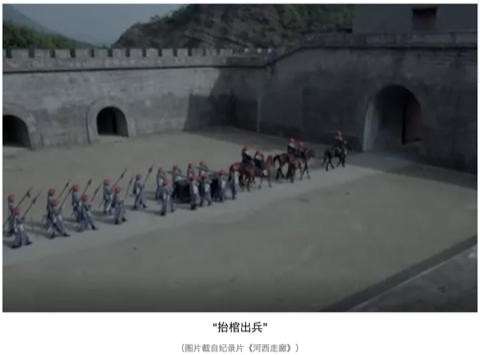
\includegraphics[width=6.67in]{images/his2}

左宗棠一定还能记起,26年前,一位即将走到生命尽头的老人与他舟中长谈,这位遍行西域三万里的老人曾大声呼吁西北边防的重要和沙俄的强烈隐患。然而,直到那晚,这位老人才在精明强干的左宗棠身上看到了可以托付边防思想的希望。

1850年11月,66岁的林则徐不甘地离开了人世。26年后,66岁的左宗棠收复了伊犁。

如果有东西可以谓之为传承,这想必便是了。

\subsection{曾国藩}

\begin{quote}
萃六州之铁,不能铸此一错
\end{quote}

曾国藩是一个以善写挽联著称的人,他曾经有一个侍妾,后来这位侍妾过世后,曾国藩写过一个挽联,里面有两句:``未必有情,对帐冷灯昏,一别竟伤春去了。''

这世间绝大多数最后没有走到一起的感情,都适用于这句话吧。未必有情,两人之间未必真的有那么深的感情,否则就可以越过世俗的一切。然而呢,一别竟伤春去了,这一别未必是生离死别,却也足够令回忆时,伤感不已。

曾国藩早年时以儒学出道,后来二次再起时兼用庄老,为官为人都到了化境。然而,却不想在天津教案上,遭遇了人生的滑铁卢。

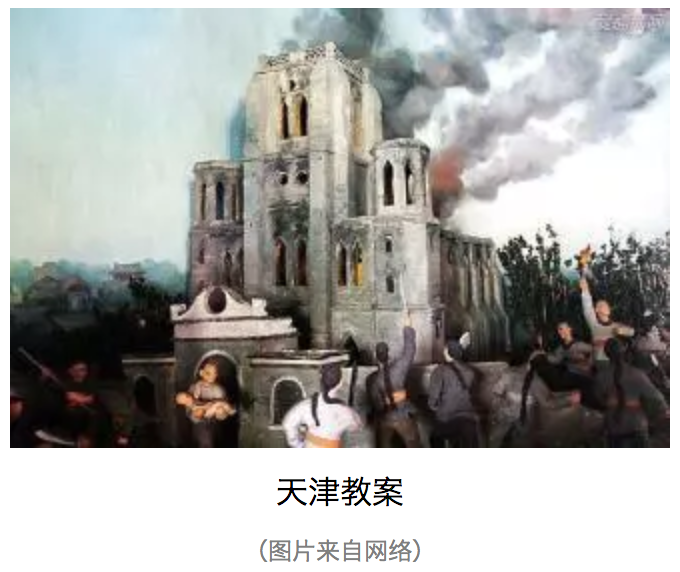
\includegraphics[width=6.67in]{images/his3}

天津教案上到底谁有错在先,已经很难分辨了,但分析史料,我们的责任恐怕还要居多。教会不管有没有错,都成为了中国人民发泄对洋人愤恨的窗口。政府的无力和国家的贫弱,成了压在人民心口挥之不去的阴影,于是捕风捉影便让20余位法国人和30余位中国信徒命丧黄泉。如果说那些持枪威胁,飞扬跋扈的外国领事死不足惜,可是剩下几十位无辜人的性命又该如何说清?

身为直隶总督的曾国藩,力排主战派的意见,首先以死囚替换成凶手,为这起事件买单;然后和天津知府张光藻、知县刘杰谈心,先行流放平息舆论,将来留做后用;最后赔偿法国损失:46万两白银(对比庚子赔款4亿五千万两)。曾国藩的处理不得当吗?不,处理的合情合理,也恰到好处。然而他却忽略了最重要的一件事情,那就是中国人民的魂。

是的,中国几千年历史沉淀下来,就像一个大染缸,谁进去都很难独善其身;是的,中国人喜欢窝里斗,喜欢贪小便宜,还麻木不仁;可是这个泱泱大国矗立在东方几千年间始终未曾间断它的历史,就一定有他的原因。这个民族的人有魂,他们在大部分时间里沉默,也终会在一个瞬间爆发出来,这足以去改变历史。虽然天津教案爆发的方式不对,但这件事情已经折射出那个时代背景下人们迫切想要去打破封建和外来殖民双重压迫的意愿,而这样的历史潮流是无法阻挡的。

所以当张光藻和刘杰被发配的时候,天津人民自发相送,人山人海,宛如送别自己的英雄。此时,即将被舆论扣上卖国贼帽子的曾国藩已经预感到自己一生的清誉将尽毁于此,不禁一声叹息:

\textbf{``萃六州之铁,不能铸此一错!''}

初读此句时,曾隔越时空,给我以强烈的震撼。这一句话也改观了我对曾国藩一生的看法。

他原名叫曾子城,后来自己改为国藩,号涤生。为国藩篱、涤尽众生!也许今天我们跳出在历史之外看他们当时做的努力似乎都无关痛痒,但局限于特定历史格局里的曾国藩却的确在用一生实践着他的名和号。天津案后两年,曾国藩与世长辞。

那位曾经不可一世且后来与曾国藩交恶到无以复加的左宗棠赠挽联写道:

\begin{quote}
知人之明,谋国之忠,自愧不如元辅
\end{quote}

\begin{quote}
同心若金,攻错若石,相期无负平生
\end{quote}

这一刻,是失去惺惺相惜之人的落寞吧,不管是曾经的朋友还是后来的对手。

\subsection{李鸿章}

\begin{quote}
秋风宝剑孤臣泪,落日旌旗大将坛
\end{quote}

太祖曾说:余于近人,独服曾文正。但我总觉得这中间少不了出自湖南的同乡之嫌;因此身为安徽人,我一直都试图去理解这位``合肥''宰相。

李鸿章在征讨捻军时实现了自己的独当一面,后来天津教案事件后,接任老师出任直隶总督,完成了权力上的接替,同时接替的,还有后来那无数的外交事宜。李鸿章一生大大小小的条约签了三十几个,如果说胡林翼留下的是虚名;左宗棠留下的是美名;曾国藩留下的是盛名;李鸿章却是实实在在背负了后来所有的骂名。

在我小的时候一直不能想明白一件事情,有一个叫美利坚合众国的国家,他们建国了两百多年,是一个从殖民地独立的国家,因此特别地强调民主与自由。在晚清时候,美国正从世界的另一端兴起,一个如此民主的国度,也有能力左右世界格局,为什么不能像春秋时候的霸主那样来维持正义呢?如果说鞭长莫及,那为什么还要加入到侵略者的队伍里去呢?后来我明白,无论是国家、家庭还是个人,不自己努力而把希望寄托于他人身上,永远是一件很可悲的事情。因为嘴上标榜的和实际去做的,常常相去甚远。

李鸿章就犯了这个错误,他过度相信了和伊藤博文这个一生之敌的友情,也错误地低估了沙俄喂不饱的野心。

北洋水师是命运跟李鸿章开的一个笑话,他像爱惜自己的孩子一样爱惜着这支队伍,可是过度的溺爱却最终导致了它的覆亡。当他让自己的心腹、不懂水军的丁汝昌作为水师提督的时候,北洋水师在很多人眼中便成为了另一个淮军。于是翁同龢老师傅在后来的过程中,对北洋水师的供给百般刁难:颐和园要翻修了,哪有那么多的钱再给到你李鸿章的水师里?于是这支建造时属于世界先进水准的水师,在七年后的甲午中日战争中已然全面落后于对手。技术的革新是一种无形的力量,一旦被淘汰,就再也追赶不上了。李鸿章太了解后来的现状,不忍心这支队伍损失太大,寄希望于调停,尽量避免主力对决,龟缩于港口,却给了对手合围全歼的机会\ldots{}\ldots{}不论如何,1895年,李鸿章创办北洋水师的功与过都已经在血与火中灰飞烟灭了。但我们仍然需要记住的是,水师提督丁汝昌、管带邓世昌以及北洋的那些将士们,他们仍然奋战到了生命的最后一刻。

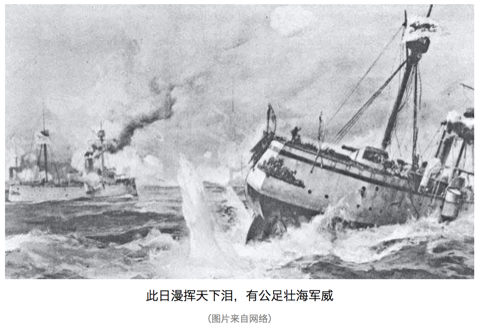
\includegraphics[width=6.67in]{images/his4}

那以后的李鸿章,像他的老师一样,舆论成为朝廷制衡他们的最好的工具,需要时就重新启用,不用时,便顺应民意罢免。后来舆论压力太大,李鸿章只好借出访海外暂避风头,想不到他在国外竟然享有比在国内更高的名誉,这不能不说是一种悲哀。然而现在就好了吗,一个已经被诺贝尔奖认可的科学家,在国内还混不到一个某某学者或者院士,这就是进步了吗?历史从来都不会消失,它们只是换了一个面孔,不停地上演。

1901年,俄国人还在步步紧逼,这位即将年满80岁的老人却已然行将就木,人之将死,其言也善,弥留之际,老人喃喃道:

\begin{quote}
劳劳车马未离鞍,临事方知一死难。
\end{quote}

\begin{quote}
三百年来伤国步,八千里外吊民残。
\end{quote}

\begin{quote}
\textbf{秋风宝剑孤臣泪,落日旌旗大将坛。}
\end{quote}

\begin{quote}
海外尘氛犹未息,诸君莫作等闲看。
\end{quote}

切莫管宰相合肥天下瘦,李鸿章是想为这个国家做出一些改变的,只是无法触及到根本,结果一生都在跟内外妥协。跟左宗棠相比,他性格中少了一些刚强;跟曾国藩相比,他头顶上少了一些神明。在李鸿章死后的第十年,清王朝连同两千多年的封建帝制一起轰然倒塌。

我最喜欢的词人辛弃疾有名句:``道男儿到死心如铁,看试手,补天裂!''当封建势力和帝国列强两头撞向不周山时,中国的天已然千疮百孔。

这天,很多人去补过,李中堂一定是其中之一。

然而中堂失败了,中正也失败了,太祖却成功了。

李鸿章曾在面对伊藤博文的嘲讽时,问道,倘若我们易地而处会如何?伊藤博文回答道,倘若易地而处,你不会比我差,而我却未必能如你。是时耶?运耶?命耶?

唉,时来天地皆同力,运去英雄不自由!

\subsubsection*{站长自述}
\addcontentsline{toc}{subsubsection}{站长自述}

科研时候搬砖,闲来无事读史,兴有所致填词。偶有``花开本无声,花落亦无痕,无可寻迹处,谁解听花人?''四句,乃谓书房听花榭。有逸闻趣事、论史谈词,入归听花杂记。又因喜闻乐见,好传八卦,人送外号广播站站长。

作者:广播站王站长 编辑:栟

\section{\texorpdfstring{真实的谎言------``何不食肉糜?''}{真实的谎言------何不食肉糜?}}

\subsection{引言}

\begin{quote}
及天下荒乱,百姓饿死,帝曰:``何不食肉糜?''其蒙蔽皆此类也。------《晋书·帝纪四惠帝》
\end{quote}

每个人都生活在特定的圈子里,这个圈子会塑造我们的世界观、人生观和价值观,进而决定了我们对事物的认知。正如王国维先生说的``以我观物,万物皆着我之色彩''。

``何不食肉糜?''是西晋晋惠帝的名言,也是长期以来大家认为他是一个白痴的铁证。但是当我们将王国维先生的观点作为一种方法论去认识晋惠帝时,也许会看到另一番图景。

\subsection{晋惠帝------活在另一个世界的帝王}

首先来分析晋惠帝的圈子和人生观,晋惠帝九岁时被正式立为太子,
``(泰始)三年春正月丁卯,立皇子衷为皇太子''。晋惠帝所处的圈子是达官显贵。而当时晋国的达官显贵们过着怎样的生活?

晋武帝每天坐着羊车找妹子,``多内宠,平吴后,复纳吴王孙皓宫人数千,自此掖庭殆将万人,而并宠者甚众,帝莫知所适,常乘羊车,恣其所之,至使宴寝。''大臣何曾每天吃饭用一万钱,还``无处下箸'';何劭一定要吃四方畛异,一天膳费二万钱;``王恺以饴澳釜'';``石崇以蜡代薪''。虽然用现在的眼光看,这是一种奢侈,可是对于一个从小生活在这样环境里的人而言,这就是生活,这就是整个世界:到处美女如云,河水里都是美酒,满山遍野都是珍馐美味,这样的世界里怎么可能有饿殍遍野?吃不上饭时``何不食肉糜?''有什么问题呢?所以他不是白痴,只是天真,只是和我们生活在不同的不同的世界。

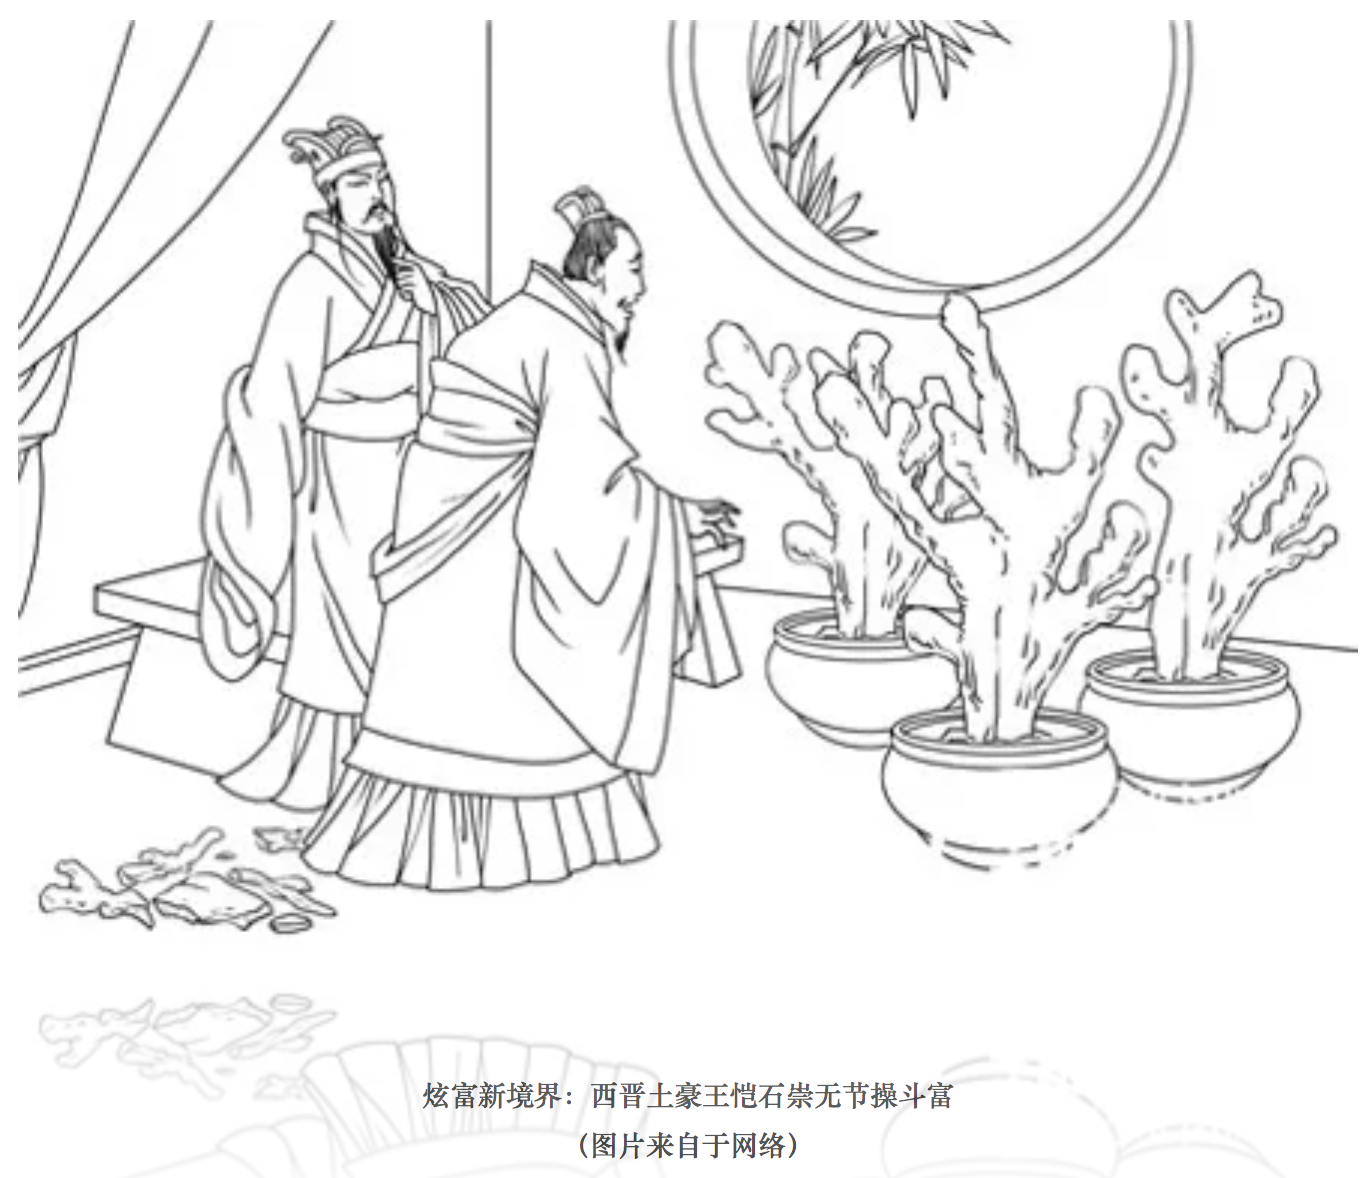
\includegraphics[width=6.67in]{images/his5}

\subsection{皇位------黄金牢笼}

建立在九品中正制之上的西晋,世家大族成为了西晋政府的实际支配者,在一个已经专制了六百多年的国家,皇权与大族之间存在着天然的矛盾,二者无法并存。世家大族为了维护自身的利益,必须限制皇权,限制皇权最好的办法莫过于打造一个对自己有利的皇帝,完成这一点必须为皇帝打造一个虚幻世界,在潜移默化中将皇帝变成自己的傀儡,这种方法在现代被称为打造文化软实力。

皇帝是几千年来中国最有权势的人,但是他们也是最可怜的人,正如钱穆先生所言,专制体制使看似高高在上的帝王落入恐惧的深渊。他们不敢与臣民直接接触,只能通过大臣来联系世界,大臣成了皇帝的耳朵和眼睛。在掌握了皇帝的耳朵和眼睛之后,大臣们可以很轻松的为皇帝打造一个楚门的世界。

回到晋惠帝的例子,晋惠帝虽然不傻,但是毕竟太天真,世界观与正常人不同,绝对不符合一个帝王的要求。对于这一点他的父亲------晋武帝很明白,至少在最初很明白,``(惠)帝之为太子也,朝廷咸知不堪政事,武帝亦疑焉。''一个``不堪政事''的太子对于皇权是一种灾难,但是对于世家大族来说是一种福音。所以``朝廷''开启了拯救``天真太子''的行动。晋书记载了一次晋武帝对太子的考核:

\begin{quote}
尝悉召东宫官属,使以尚书事令太子决之,帝不能对。贾妃遣左右代对,多引古义。给事张泓曰:「太子不学,陛下所知,今宜以事断,不可引书。」妃从之。泓乃具草,令帝书之。武帝览而大悦,太子遂安。
\end{quote}

虽然《晋书》里只是寥寥数语,但是这几个字却透露出阵阵寒意。既然是考核,而且是``以尚书事''即处理正常公务来考核,晋武帝就不可能将题目提前交给晋惠帝,根据这段记录很明显晋惠帝事先获得考题。这表明晋惠帝身后的利益集团可以掌握晋武帝现在的想法(拿到考题);未来的想法(不能临时加题);对事物的判断(回答的分寸拿捏必须准确,既要不能完美到让晋武帝起疑又不能太差),能同时做到以上几点,无疑表明大臣们已经成功将皇帝至于自己精心打造的世界里。

虽然史料里只记载了一次考核,但是我们有理由相信,对于皇位继承人,考核一定不只一次。每一次通过都很困难,但是晋惠帝都通过了,只能表明这个世界的禁锢是多么严密。连平吴代魏的晋武帝都无法逃脱楚门的世界,更不用说晋惠帝。所以从体制上晋惠帝只能生活在自己的世界里,无法与正常人有相同的世界观。

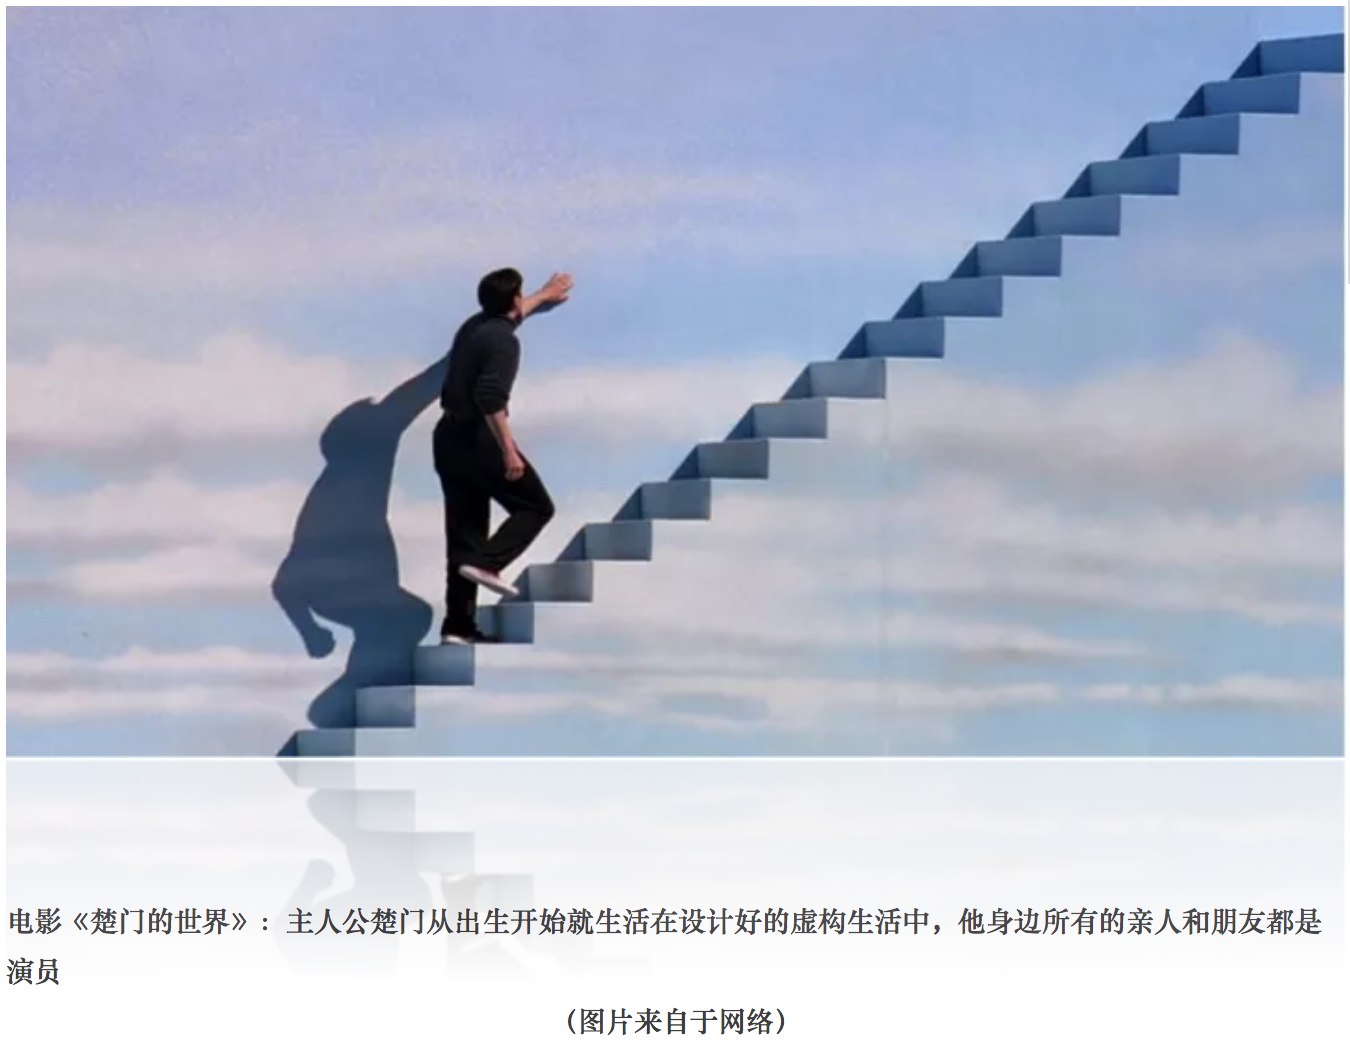
\includegraphics[width=6.67in]{images/his6}

\subsection{枕边人------妻管严的悲哀还是家有贤妻的明智}

史书都是由后人书写,人们往往倾向于做事后诸葛亮。正如做题一样,一道题我们百思不得其解,但是当我们看过答案之后,再来审视这道题,我们就会发现题目里处处是线索。明确了这一点之后,我们就又可以回到晋惠帝的故事了。《晋书》对晋惠帝的评价是``不才之子,则天称大,权非帝出,政迩宵人。''认为晋惠帝不仅本身能力有问题,还管不住自己的老婆,所有的坏事都是他的皇后干的。

这个观点貌似似曾相识,周幽王是昏庸,但是西周灭亡的直接责任人是褒姒;纣王是无道,但是主要原因是妲己;李自成是能力欠佳,但是快速败亡和陈圆圆脱不了干系。女人真是史学家的真爱,隔不多时就要被拿出来当挡箭牌。

鉴于此,不得不好好说一说晋惠帝的皇后------贾南风,西晋功臣贾充之女。贾南风其人,貌似对她的记载几乎都落在了如下几个批语上``妒而少子、丑而短黑、荒淫放恣。''首先说这个丑字,不太好考证,但是我看到了如下关于她妹妹的记录:

\begin{quote}
(贾午)婢后往寿家,具说女意,并言其女光丽艳逸,端美绝伦。寿闻而心动,便令为通殷勤。婢以白女,女遂潜修音好,厚相赠结,呼寿夕入。
\end{quote}

大意是说贾午看上了一个自己父亲的属官叫韩寿,然后让婢女去和他表达了希望交往的意愿,并且说自己有多好看,然后他们就幸福的在一起了。这个韩寿不太可能是贪图贾氏的权力,因为他本身也是达官显贵之后,曾祖父做过魏国高官,同时采用私通长官女儿的方式获得权力,怎么看都有点作死,要是直接私通贾充还可以理解。所以这个故事表明,贾午至少不难看,作为同父同母的姐姐,我觉得上帝不会太不公平吧。

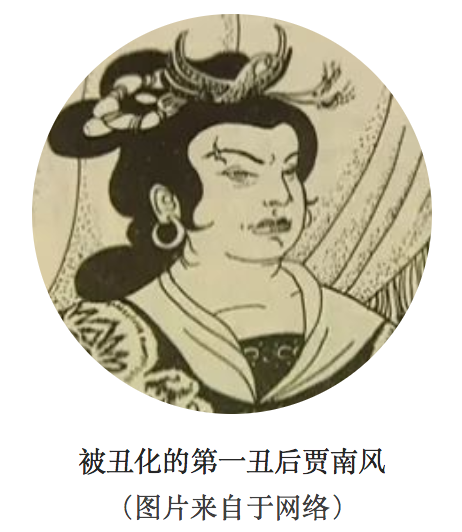
\includegraphics[width=5.79in]{images/his7}

从政治角度而言,贾南风在晋惠帝即位后联络司马玮、司马亮杀杨骏,废杨太后;然后又让司马玮杀司马亮和卫瓘;最后又杀掉了司马玮。杨骏何许人也?杨骏的妹妹是当时的皇太后,对于外朝,杨骏``为太傅、大都督、假黄钺,录朝政,百官总己''
可谓权倾朝野;对于内朝,``虑左右间己,乃以其甥段广、张劭为近侍之职'',安插自己人为``近侍之臣'',宋太祖有句话叫``卧榻之旁岂容他人酣睡'',杨骏的做法已经是要看着晋惠帝入睡了。

这样的权臣想必晋惠帝和贾南风都不会陌生,已经安躺在司马家祖庙里的几位先人可不比杨骏差。所以无论新登基的是谁,杨骏都是必然会被清理的政治力量。这样来看这个故事是不是似曾相识?

东汉末年,大将军何进让董卓铲除宦官。结果没想到自己先被宦官狗带了,真是自己驱虎吞狼却先被狼吃了。这样一对比,晋惠帝和贾南风驱虎吞狼,最后把狼和虎一起给炖了,这样的政治手腕腻不腻害,高不高明?

就私生活而言,她的父亲出过轨,妹妹出过轨,所以在这样的家庭长大,她出轨的概率确实高于常人,但是这并不是她是一个坏的政治家的理由。但其实,纵看几千年的历史,你以为皇帝后宫里能有几个贞节牌坊么?

综上来看,对于一个这样的皇后,晋惠帝让她放手做一些事情好像并没有太大的问题。

\subsection{结语}\label{-2}

怀疑论者曰:晋惠帝是一个生活天真的,与大众生活在不同世界的帝王,他的工作特点使他没机会与大众生活在同一个世界。婚后,对爱人的工作能力予以充分的肯定,取得了一定的工作成绩,但是由于工作能力不足最终导致了工作单位倒闭。

\subsubsection*{作者简介}
\addcontentsline{toc}{subsubsection}{作者简介}

初以科研为业,现守朱门。喜忆往昔风云人物,多有异见,然无意见。欲起一笔名,思虑万千,终觉yy最为妥帖。

作者:yy 校稿:广播站王站长 编辑:智公子 图片:柴胡半夏苏

\bibliography{book.bib}


\end{document}
